% Options for packages loaded elsewhere
\PassOptionsToPackage{unicode}{hyperref}
\PassOptionsToPackage{hyphens}{url}
%
\documentclass[
  12pt,
]{article}
\author{}
\date{\vspace{-2.5em}}

\usepackage{amsmath,amssymb}
\usepackage{lmodern}
\usepackage{iftex}
\ifPDFTeX
  \usepackage[T1]{fontenc}
  \usepackage[utf8]{inputenc}
  \usepackage{textcomp} % provide euro and other symbols
\else % if luatex or xetex
  \usepackage{unicode-math}
  \defaultfontfeatures{Scale=MatchLowercase}
  \defaultfontfeatures[\rmfamily]{Ligatures=TeX,Scale=1}
\fi
% Use upquote if available, for straight quotes in verbatim environments
\IfFileExists{upquote.sty}{\usepackage{upquote}}{}
\IfFileExists{microtype.sty}{% use microtype if available
  \usepackage[]{microtype}
  \UseMicrotypeSet[protrusion]{basicmath} % disable protrusion for tt fonts
}{}
\usepackage{xcolor}
\IfFileExists{xurl.sty}{\usepackage{xurl}}{} % add URL line breaks if available
\IfFileExists{bookmark.sty}{\usepackage{bookmark}}{\usepackage{hyperref}}
\hypersetup{
  hidelinks,
  pdfcreator={LaTeX via pandoc}}
\urlstyle{same} % disable monospaced font for URLs
\usepackage[margin=1in]{geometry}
\usepackage{longtable,booktabs,array}
\usepackage{calc} % for calculating minipage widths
% Correct order of tables after \paragraph or \subparagraph
\usepackage{etoolbox}
\makeatletter
\patchcmd\longtable{\par}{\if@noskipsec\mbox{}\fi\par}{}{}
\makeatother
% Allow footnotes in longtable head/foot
\IfFileExists{footnotehyper.sty}{\usepackage{footnotehyper}}{\usepackage{footnote}}
\makesavenoteenv{longtable}
\usepackage{graphicx}
\makeatletter
\def\maxwidth{\ifdim\Gin@nat@width>\linewidth\linewidth\else\Gin@nat@width\fi}
\def\maxheight{\ifdim\Gin@nat@height>\textheight\textheight\else\Gin@nat@height\fi}
\makeatother
% Scale images if necessary, so that they will not overflow the page
% margins by default, and it is still possible to overwrite the defaults
% using explicit options in \includegraphics[width, height, ...]{}
\setkeys{Gin}{width=\maxwidth,height=\maxheight,keepaspectratio}
% Set default figure placement to htbp
\makeatletter
\def\fps@figure{htbp}
\makeatother
\setlength{\emergencystretch}{3em} % prevent overfull lines
\providecommand{\tightlist}{%
  \setlength{\itemsep}{0pt}\setlength{\parskip}{0pt}}
\setcounter{secnumdepth}{-\maxdimen} % remove section numbering
\newlength{\cslhangindent}
\setlength{\cslhangindent}{1.5em}
\newlength{\csllabelwidth}
\setlength{\csllabelwidth}{3em}
\newlength{\cslentryspacingunit} % times entry-spacing
\setlength{\cslentryspacingunit}{\parskip}
\newenvironment{CSLReferences}[2] % #1 hanging-ident, #2 entry spacing
 {% don't indent paragraphs
  \setlength{\parindent}{0pt}
  % turn on hanging indent if param 1 is 1
  \ifodd #1
  \let\oldpar\par
  \def\par{\hangindent=\cslhangindent\oldpar}
  \fi
  % set entry spacing
  \setlength{\parskip}{#2\cslentryspacingunit}
 }%
 {}
\usepackage{calc}
\newcommand{\CSLBlock}[1]{#1\hfill\break}
\newcommand{\CSLLeftMargin}[1]{\parbox[t]{\csllabelwidth}{#1}}
\newcommand{\CSLRightInline}[1]{\parbox[t]{\linewidth - \csllabelwidth}{#1}\break}
\newcommand{\CSLIndent}[1]{\hspace{\cslhangindent}#1}
\usepackage{setspace}
\doublespacing
\usepackage{lineno}
\linenumbers
\usepackage[belowskip=0pt,aboveskip=0pt]{caption} \usepackage{array} \usepackage{caption} \usepackage{graphicx} \usepackage{siunitx} \usepackage{colortbl} \usepackage{multirow} \usepackage{hhline} \usepackage{calc} \usepackage{tabularx} \usepackage{tabulary} \usepackage{threeparttable} \usepackage{wrapfig}
\usepackage{booktabs}
\usepackage{longtable}
\usepackage{array}
\usepackage{multirow}
\usepackage{wrapfig}
\usepackage{float}
\usepackage{colortbl}
\usepackage{pdflscape}
\usepackage{tabu}
\usepackage{threeparttable}
\usepackage{threeparttablex}
\usepackage[normalem]{ulem}
\usepackage{makecell}
\usepackage{xcolor}
\ifLuaTeX
  \usepackage{selnolig}  % disable illegal ligatures
\fi

\begin{document}

\newpage

\hypertarget{estimating-population-trends-under-the-pressures-of-climate-change}{%
\section{Estimating Population Trends Under the Pressures of Climate Change}\label{estimating-population-trends-under-the-pressures-of-climate-change}}

Benjamin A. Levy\textsuperscript{1}, Christopher M. Legault\textsuperscript{2}, Timothy J. Miller\textsuperscript{2}, Elizabeth N. Brooks\textsuperscript{2}

\textsuperscript{1}Ocean Associates Inc.~in support of \textsuperscript{2}National Marine Fisheries Service, Northeast Fisheries Science Center, 166 Water Street, Woods Hole, Massachusetts 02543-1026

Corresponding author: Ben Levy (\href{mailto:blevy6@gmail.com}{\nolinkurl{blevy6@gmail.com}})

Competing interests: The authors declare there are no competing interests.

\newpage

\hypertarget{abstract}{%
\subsection{Abstract}\label{abstract}}

Many stock assessments in the United States use biomass estimates derived from stratified random bottom trawl data. To accurately track changes in true biomass of a species, catch observations must contain low noise and the proportion of the population that is sampled should be consistent over time. One increasingly documented phenomenon that violates the latter assumption is climate-induces movement leading to changes in relative biomass between sampled and unsampled portions of the stock area. Using the R package MixFishSim, we have developed data-driven spatial models for Yellowtail Flounder, Atlantic Cod, and Haddock in the western Atlantic Ocean to evaluate two methods of estimating population trend given temperature driven movement. Movement rates combine species-specific static habitat preferences with temperature tolerances. Habitat preferences were derived from niche models relating bottom trawl catches to environmental covariates. A repeating yearly temperature pattern produces repeating spatial biomass distributions in a given week, while a temperature gradient that increases on average over time results in spatial preferences that evolve throughout a given simulation. We simulated spatial time series data sets for each species for several temperature scenarios and population trends. Using stratified random sampling on model output we were able to compare biomass estimates derived from the design-based stratified mean to those using a spatio-temporal model-based approach that allows inclusion of environmental covariates. Our focus was on the ability of contemporary index standardization methods to track population trends under shifting spatial preferences.

\hypertarget{keywords}{%
\subsection{Keywords}\label{keywords}}

survey, design-based, model-based, climate change, population simulation, VAST

\newpage

\section{Introduction}

The continental shelf off the coast of the Northeast United States spans from the Outer Banks of North Carolina to the Gulf of Maine. The region covers over 250,000 km\(^2\) of ocean, extending over 200 km from shore in the largest areas in New England to just 30 km off shore in the southern regions. This ecologically diverse region contains approximately 18,000 vertebrate marine species, making commercial fisheries an important part of local economies for centuries. In 2019, New England fisheries produced \$22 billion in sales, which supported over 200,000 jobs ({``{Fisheries Economics of the United States: Data and Visualizations}''} n.d.). Maintaining a healthy ecosystem is therefore vital to the economic prosperity of the region.

The Northeast Fisheries Science Center (NEFSC) has conducted a bottom trawl survey since 1963 to support assessment and management of the fish and invertebrate populations in the region (Azarovitz 1981; Politis et al. 2014). The survey uses a stratified random design where bottom trawl sampling takes place in predefined strata along the eastern continental shelf, where depth and latitude define the strata. The survey has created a rich time series data set with many uses including species-specific habitat identification, age and life history information, analysis of how environmental conditions influence species biomass, and estimating yearly species biomass trends to help inform stock assessments, and ultimately fishing quota limits. The survey takes place twice each year- once in the spring and again in the fall. Most spatial analyses and projections of future distributions typically assume a constant survey catchability and availability over time. For this reason, NOAA's survey design includes sampling each stratum in approximately the same 6 week time period in each season.

One component of a stock assessment is an estimation of yearly biomass that is often derived from the bottom trawl survey, when applicable. Stock assessment scientists choose from a number of approaches to obtain biomass estimates ranging from traditional design-based estimates to model-based estimates that vary in complexity. Design-based estimators rely on the design of the sampling scheme with the underlying assumption that the data being collected is representative of the population of interest. These methods typically account for spatial variation in samples by stratifying the sampling area. While it is possible to include environmental influences with design-based methods (Deville and Särndal 1992), it is not a common practice. Model-based biomass estimates use statistical models to measure the relationship between response variables (such as presence or biomass) and predictor variables (such as environmental factors). Model-based estimators help account for complex relationships between variables and can help overcome problems related to the sampling process. Common model-based approaches include Generalized Linear Models (GLM), Generalized Additive Model (GAM), and General Linear Mixed Models (GLMM).

Due to a combination of climate change and shifts in circulation, the Northeast United States continental shelf has experienced rapid warming in recent decades. At the same time a number of recent studies have found a shift in spatial distributions of many species (Nye et al. 2009; Henderson et al. 2017; Kleisner et al. 2017). Since stock assessment models rely on accurate descriptions of population dynamics and contemporary patterns of spatial abundance, there is concern that rapid undocumented changes in spatial distributions of species will bias future stock assessments. More specifically, as fish populations shift their distributions over time, catchability and/or availability in the survey could change, altering the relationship between the index and the true population (Arreguı́n-Sánchez 1996; Langan et al. 2021). A species shifting its range beyond the survey area or outside of the assumed stock boundary is an additional compounding factor to consider. Existing research has focused on temperature as the driver of such changes (Klein et al. 2017) and evidence suggests that failing to account for the impact of climate-induced change can lead to management challenges (Kerr et al. 2022). In these scenarios, management strategy evaluations have shown that misconceptions of stock status can lead to unintended overfishing, which can ultimately have detrimental ecologic and economic impacts (Mazur et al. 2023). We are therefore interested in analyzing the impact of climate driven movement and distribution changes on the accuracy of biomass estimates derived from NOAA's ongoing bottom-trawl survey along the east coast.

To test the ability of the bottom trawl survey to track population trends under shifting environmental conditions, we construct spatial models for fish where movement depends on temperature preferences. We consider the impact of climate change by comparing simulations that use a repeating water temperature pattern to those where temperature increases on average over time. In both cases we conduct stratified random sampling (SRS) on model output and analyze the ability of the samples to track population trends. We compare yearly biomass estimates obtained from the stratified mean to estimates obtained from the Vector-Autoregressive Spatio-temporal (VAST) model. The stratified mean is a design-based approach that calculates the stratum specific mean catch per tow, which are then weighted by stratum area to obtain an overall mean. VAST is a spatial delta-generalized linear mixed model that estimates both biomass and probability of occurrence (presence/absence) (Thorson 2019). VAST also allows users to include covariate data to better inform the model. Covariates can be static (e.g.~habitat preferences) or dynamics (e.g.~temperature). We explore whether including environmental predictors leads to improved biomass estimates, which is particularly relevant as climate change progresses.

\section{Methods}

We construct spatial population models for Yellowtail Flounder (\emph{Limanda ferruginea}), Atlantic Cod (\emph{Gadus morhua}), and Haddock (\emph{Melanogrammus aeglefinus}) on Georges Bank, hereafter referred to as Yellowtail, Cod, and Haddock. Movement of each species combines static species-specific habitat preferences with biologically-based temperature preferences. Model dynamics are driven by a time series of temperature gradients to create simulated spatial data sets for each population where the true biomass is known. Using temperature gradients that repeat each year creates data sets with repeating spatial patterns, whereas using a temperature gradient that increases on average throughout the simulation leads to spatial distributions that shift over time. We conduct SRS on our simulation data to mimic the bottom trawl survey and use the samples to compare the ability of contemporary index standardization methods to track population trends.

\subsection{Population Model Formulation}

We use the R package \emph{MixFishSim} (MFS) to model our populations (Dolder et al. 2020). MFS is a discrete spatiotemporal simulation tool that allows users to model multiple species under varying environmental conditions. The package uses a delay-difference population model with discrete processes for growth, death, and recruitment of the population. To address our research question we specify the following inputs for the MFS package.

\emph{Study Area}

A shapefile for the 15 strata that comprise Georges Bank was discretized into a raster with 88 rows and 144 columns to use as our modeling environment. Each cell in our simulation domain represents approximately 8.7 km\(^2\). A fish stock is considered to be a subpopulation of a species that has similar intrinsic parameters. Each of the species being modeled has multiple biologically distinct stocks along the Atlantic coast resulting from local environmental conditions. As a result, each stock inhabits a different number of strata on Georges Bank. Haddock inhabit all 15 strata in the domain, Cod populate 13 strata, and Yellowtail can be found in 9 strata (Figure \ref{fig:strata-plot}).



\begin{figure}

{\centering 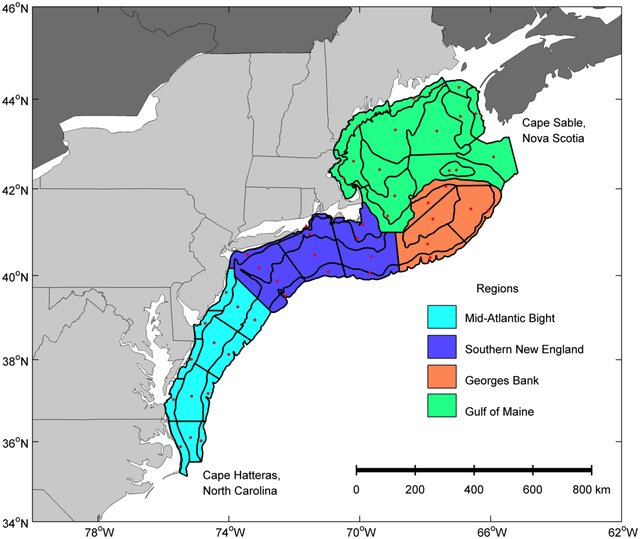
\includegraphics[width=0.95\linewidth]{Images/GB_strata} 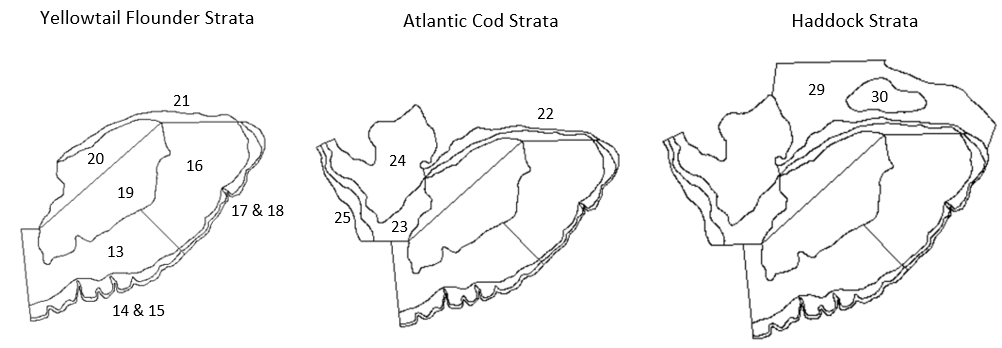
\includegraphics[width=0.95\linewidth]{Images/Strata2} 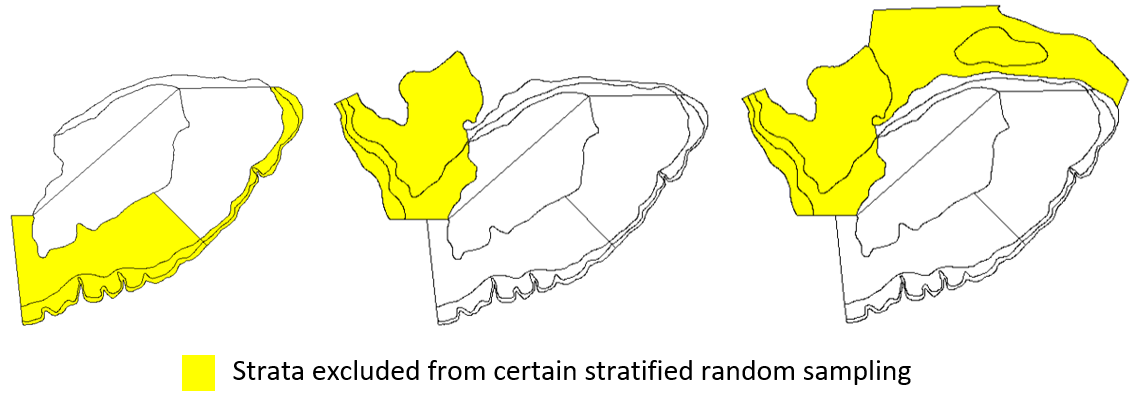
\includegraphics[width=0.95\linewidth]{Images/Excluded_strata2} 

}

\caption{Strata inhabited by each species in our population models. All strata on the eastern US contintental shelf are shown in the first image with Georges Bank highlighted in orange (Walsh et al. 2015). Stratum numbers used by the NEFSC bottom trawl survey are shown in the middle row. Strata that are excluded from certain stratified random sampling are shown in the bottom row in yellow.}\label{fig:strata-plot}
\end{figure}

\emph{Population Dynamics and Recruitment}

The time step for our models is one week. MFS uses a modified two-stage Deriso-Schnute delay difference equation that models the biomass in each cell in our study area (Dolder et al. 2020). Parameters in the population model account for growth of mature adults, mortality (natural and fishing), and the addition of new recruits. Recruitment is a function of the adult biomass that existed in the previous year and is added to the population incrementally throughout each species' predefined spawning period. Parameter inputs were either obtained from the literature or chosen to produce desired model dynamics, and therefore, these results cannot be compared directly with stock assessment results. A full list of parameters used in our population model can be seen in Tables 1 and \ref{tab:paramsSCENARIOS}.

\emph{Movement}

The package combines species-specific temperature tolerances with habitat preferences to drive the probability of movement from cell \(I\) to cell \(J\) in week \(wk+1\) using the formulation

\begin{align}
Pr(C_{wk+1}=J|C_{wk}=I) = \frac{e^{-\lambda \cdot d_{I,J}}\cdot(Hab^2_{J,s} \cdot Tol_{J,s,wk})}{\sum^C_{c=1}e^{-\lambda \cdot d} \cdot (Hab^2_{c,s} \cdot Tol_{c,s,wk})},
\label{moveP}
\end{align}

where

\(e^{-\lambda \cdot d_{I,J}}\) accounts for distance between cells \(I\) and \(J\),

\(Hab^2_{J,s}\) is the static habitat value for species \(s\) in cell \(J\), and

\(Tol_{c,s,wk}\) is the value from normally distributed temperature tolerance for species \(s\) in cell \(c\) in week \(wk\).

The MFS package was designed to generate hypothetical temperature gradients and theoretical habitat preferences using Gaussian Random Fields. The following sections describe how we configured the habitat and temperature components to model our three species on Georges Bank.

\emph{Habitat Input}

The habitat input for each species in MFS should represent spatial habitat preferences for each species that are time-invariant and are instead related to static geographic features. Species-specific habitat preferences were derived from niche models for each species using the \emph{lrren} tool from the R package \emph{envi} (Buller 2022). The \emph{lrren} tool estimates an ecological niche using the relative risk function by relating presence/absence data to two covariate predictors. We used bottom trawl point data from 2009-2021 as our presence/absence input by using a value of 0 for any tow that failed to catch the given species and by representing a successful catch by the biomass of the given tow. We combined data from both the fall and spring surveys to obscure seasonal influences to allow the niche model to instead infer static habitat preferences independent of temperature. Depth and mean sediment size were used as our covariate predictors. Estimated depth for the region was obtained from FVCOM (Chen et al. 2006). The mean sediment size raster was interpolated in ArcMap using the natural neighbor interpolation method using point data collected by the United States Geologic Survey (USGS) (McMullen et al. n.d.). Since the values in \(Hab_{J,s}\) are required to be between 0 and 1, we rescaled the spatial estimates from \emph{lrren} to fall between these bounds. See Figure \ref{fig:hab-plot1} for a visual representation of this process being applied to Cod. Figure \ref{fig:hab-plot} depicts habitat preferences \(Hab_{J,s}\) for each species.

\begin{figure}

{\centering 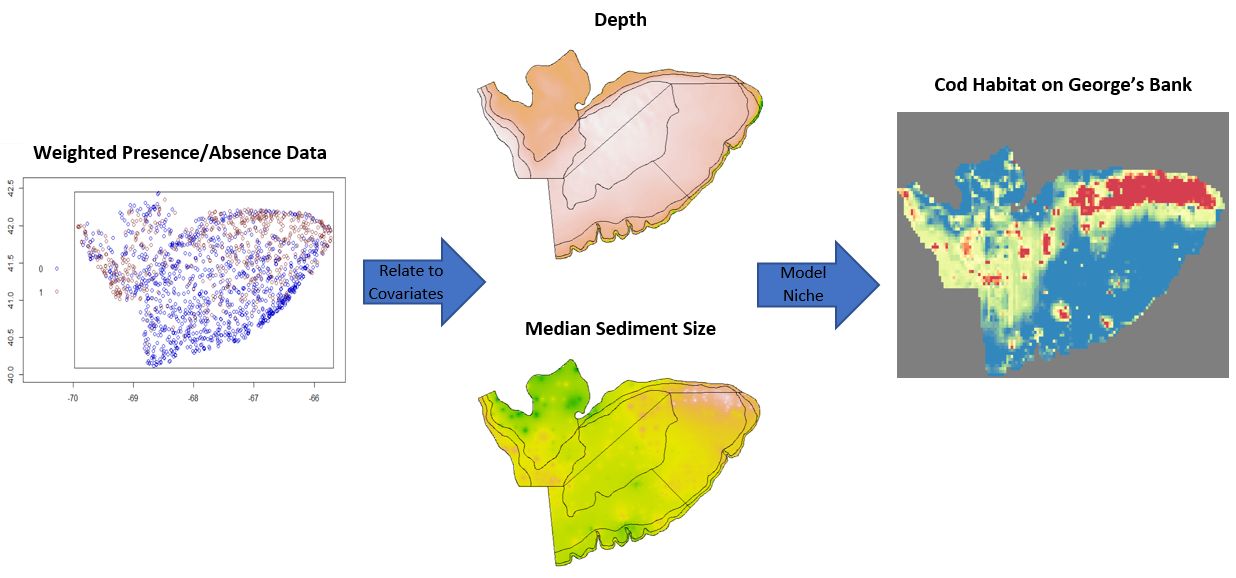
\includegraphics[width=0.95\linewidth]{Images/hab_snip3} 

}

\caption{Visual representation of niche model for Atlantic Cod. In the left most plot, tows with positive Cod catch are shown in red while tows without Cod are in blue. Positive tows are weighted by the biomass of the given catch. The middle two plots show our covariate predictors used in the \textit{lrren} niche model- depth and median sediment size. The plot on the right shows the final niche model that has been rescaled between 0 and 1, where blue values are closer to 0 and red values are closer to 1.}\label{fig:hab-plot1}
\end{figure}

\begin{figure}

{\centering 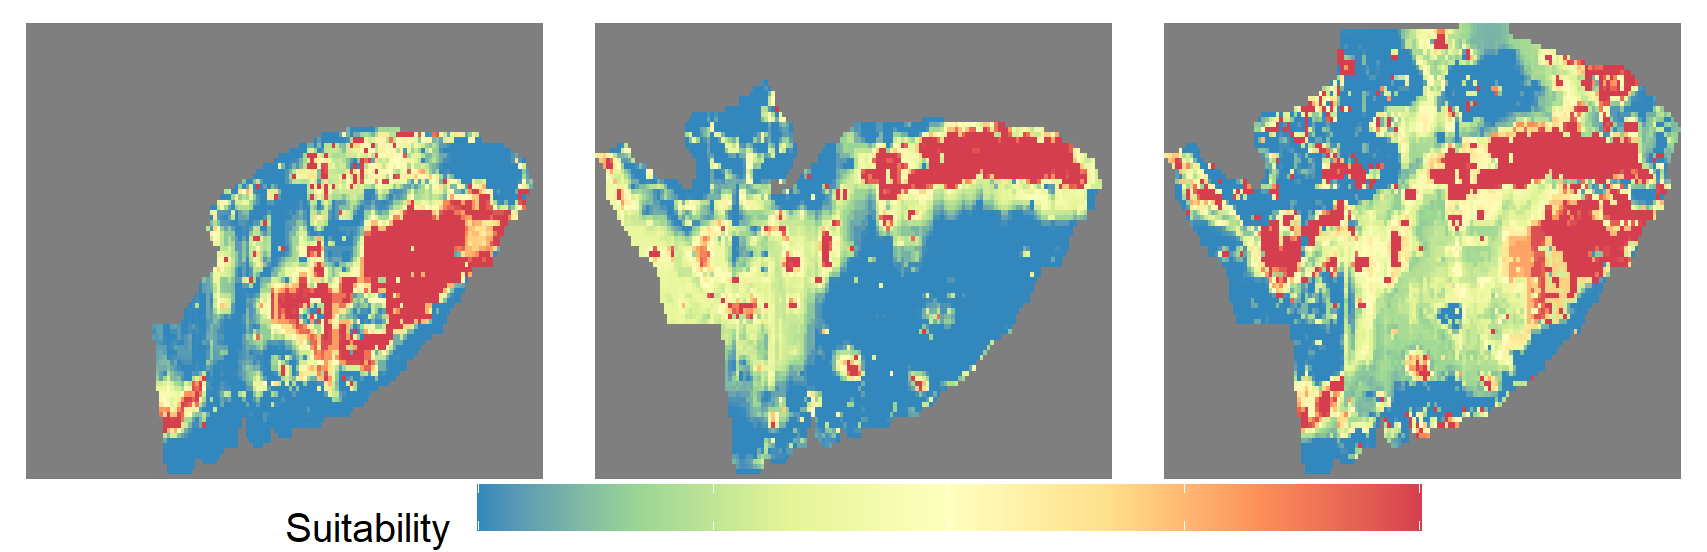
\includegraphics[width=0.95\linewidth]{Images/Habitat_3species} 

}

\caption{Static habitat preferences for each species in our population models. From left to right: Yellotwtail Flounder, Atlantic Cod, and Haddock.}\label{fig:hab-plot}
\end{figure}

\emph{Temperature Input}

Each species is assumed to have normally distributed temperature preferences \(N(\mu,\sigma)\), with mean \(\mu\) and standard deviation \(\sigma\). Temperature values are in degrees Celcius. Values were chosen by combining information in the literature with temperatures recorded in the bottom trawl survey. We assume Yellowtail's preferences are \(N(8.75,4.25)\), while Haddock and Cod have preferences \(N(9,4)\). Weekly estimated temperature data for the region for 2012 was obtained from FVCOM (Chen et al. 2006). We chose to repeat temperature estimates for a single year rather than use data for consecutive years to reduce the number of factors impacting model dynamics while still incorporating real data. The 2012 data was chosen because it displayed an average temperature pattern that consistently oscillated between maximum and minimum temperature values, allowing for a smooth repeating yearly temperature pattern for the constant temperature scenario. The 2012 temperature data was also transformed to create an oscillating pattern that increases 5 degrees Celsius on average over the duration of the simulation. We chose a 5 degree increase over a 20 year simulation to allow temperature change to have a meaningful impact on spatial patterns while remaining within reasonable computational limits in terms of the length of the simulation. Figure \ref{fig:temp-scenarios} depicts mean trends for the temperature scenarios used in our population models. \textbf{dont forget to include animated gif in final submission}

\begin{figure}

{\centering 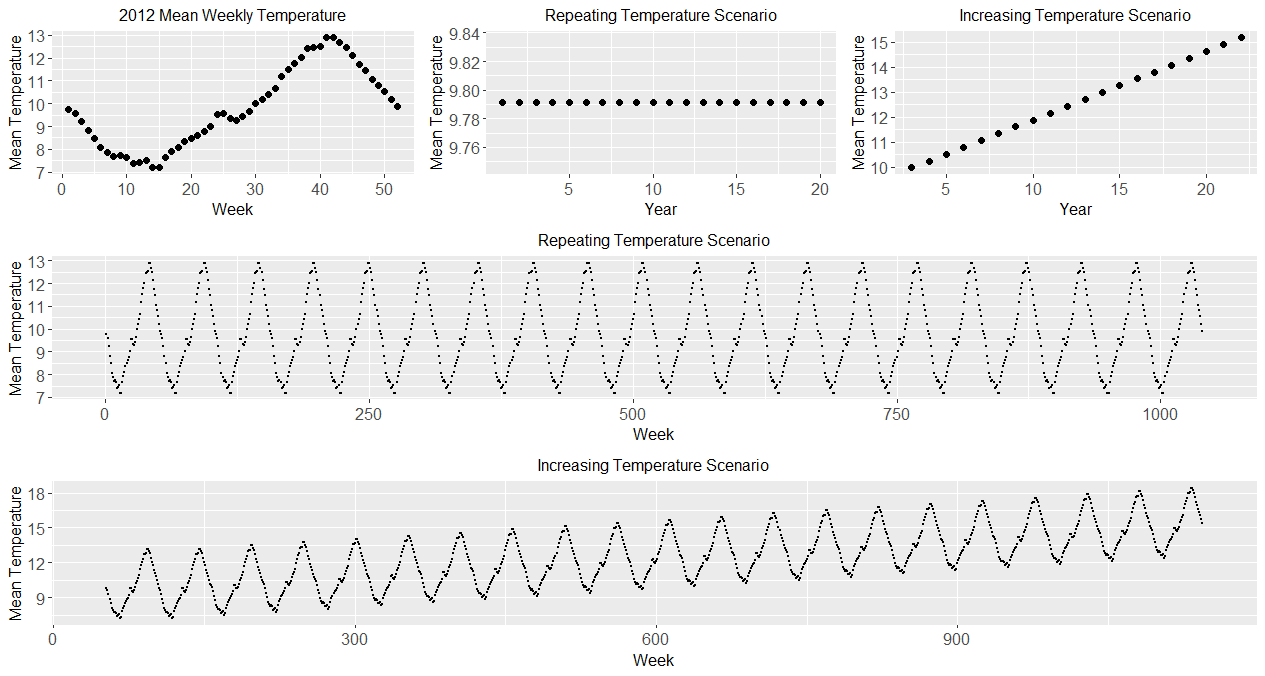
\includegraphics[width=0.95\linewidth]{Images/TempScenarios} 

}

\caption{Mean trends of temperature data used in our MixFishSim population model.}\label{fig:temp-scenarios}
\end{figure}

In equation (1), \(Hab^2_{J,s}\) remains constant for each species for the duration of the simulation, while \(Tol_{c,s,wk}\) changes each week with temperature fluctuations. Using a temperature gradient that repeats every 52 weeks produces the same spatial preferences in a given week each year, resulting in relatively consistent spatial biomass patterns. Scenarios where the temperature increases over time creates spatial preferences that evolve as the water warms, producing spatial biomass patterns that shift in a given week over the duration of the simulation.

We carry out 20 year simulations for each of our three species under various population scenarios. Historically, Cod has seen significant decline over the last 50 years while Haddock has increased in abundance in recent years ((NEFSC) 2022). For this reason we compare survey index estimates using SRS from decreasing population scenarios for Cod and increasing population scenarios for Haddock. To consider a wide range of possibilities, we include increasing, decreasing, and constant population trends for Yellowtail. The specific population trends used in our analyses can be see in Figure \ref{fig:pop-scenarios}. Each of these scenarios is simulated twice: first with with an oscillating temperature gradient that repeats and second with a temperature gradient that increases roughly 5 degrees Celsius over the duration of the 20 year simulation, for a total of 10 simulated spatial data sets.

\begin{figure}

{\centering \includegraphics[width=0.99\linewidth]{Images/Population_scenarios2} 

}

\caption{True population trends used in index analyses. Spring biomass plots are shown with fall values being very similar.}\label{fig:pop-scenarios}
\end{figure}

\emph{Simulating Bottom Trawl Survey and Population Index}

After distributing each species in its stock area with simulated population trajectories, we mimic the bottom trawl survey by conducting SRS in the set of strata associated with each stock twice each year. We sample each stratum in the same weeks in which the spring and fall surveys have historically sampled Georges Bank (weeks 13 and 14 in the spring and 37 and 38 in the fall). The number of simulated tows made reflects true target values for each stratum and sample cells where ``tows'' are made were randomly selected.

An underlying assumption in all index methods is that individual random samples combine to accurately represent true biomass by a) containing a low enough noise level in the samples to allow for a discernible pattern and b) consistently sampling the same proportion of the population. These assumptions can be questioned given enough noise in the sampling process and/or climate change causing a population to move into previously uninhabited strata. To simulate the impact of noise, we compare index estimates after adding noise to our samples versus those using the true sampling values. Annual survey observations were simulated as log-normal deviations from the underlying ``true'' survey catches with a CV of 0.35. The implication of a given population shifting its distribution into new habitat outside of the normal survey area is that SRS will fail to sample the entire geographic extent of the population. We simulate the effect of populations moving into new habitat by comparing index estimates using samples from all strata inhabited by each species on Georges Bank to those that only include a subset of the full spatial domain for each species. The strata to exclude for each species were chosen by reviewing how the distribution of each species evolved in our increasing temperature scenarios and removing strata where the proportion of a given population was changing over time. Figure \ref{fig:strata-plot} shows all strata inhabited by each species as well as those that are removed from certain calculations using the spatial shifting trends shown in Figure \ref{fig:PopPct}. The yellow regions in Figure \ref{fig:strata-plot} depict the strata that were not sampled for each species in this scenario. We then use the biomass collected from our samples in contemporary biomass index methods to estimate yearly seasonal population trends.

The design-based method we used is the stratified mean, which divides the inhabited domain into \(N\) disjoint strata based on relevant geographic and environmental information such as depth and latitude/longitude. The number of samples taken from each stratum \(S_j\) for \(j=1...N\) is proportional to the given area. The stratified mean biomass \(SM_{s,y}\) for a given season \(s\) and year \(y\) can then be calculated as the weighted average

\begin{equation*}
 SM_{s,y} = \sum_{i=1}^N W_i \frac{\sum_{k=1}^{S_i}y_{k,i}}{S_i},
\end{equation*}

where \(W_i=\frac{A_i}{\sum_{j=1}^N A_j}\), \(A_i\) is the area of stratum \(i\), and \(y_{k,i}\) represents the biomass in sample \(k\) of stratum \(i\) in season \(s\) and year \(y\). These tow-dependent calculations are quick and easy to calculate, especially relative to the model-based VAST estimates.

We compare stratified mean estimates to those derived from the model-based VAST approach. VAST models both encounter probability \(p_1(i)\) and positive catch rate \(p_2(i)\) for each observation \(i\) as linear predictors using a spatial delta-generalized linear mixed model that can be represented by

\[
  \makebox[\linewidth]{$f(p_*(i))= \beta_*(t_i) + L_{\omega_*}\omega_*(s_i) + L_* \epsilon_*(c_i,t_i) + \upsilon(s_i,t_i) + \xi(i),$}
\]

for \(*=1,2\), where more specific functional forms of each component are further described in Thorson (2019). VAST models require numerous user inputs to determine how the linear predictors will be conditioned and solved. As a result, VAST models take on the order of hours to complete.

We follow the advice given in (Thorson 2019) and \url{https://github.com/James-Thorson-NOAA/VAST/wiki} to build VAST estimates of biomass in our Georges Bank spatial population models using stratified random samples from our simulation output. In addition to exploring different link functions and assumed distributions, our VAST model-building process involved testing the impact of including spatial and/or spatio-temporal variation in our models, considering varying number of knots in our mesh, and testing different forms of temporal correlation. We carried out the same model-building process using covariate information to inform our models as well as without covariates in our models. We considered the driving factors of movement in our population models as covariates- the dynamic temperature values and static habitat values (\(Hab_{J.s}\)). We ultimately decided to provide the most information to the model by including exact values for both temperature and habitat covariates to consider a best-case scenario.

Knowing the true population values in our simulations allows us to compute the relative absolute error in a given season \(E_s\) from each estimation method and scenario as given by

\begin{equation}
E_s = \frac{\sum_{y=1}^{20}|M_{i,s}-I_{i,s}|}{\sum_{y=1}^{20}M_{i,s}},
\end{equation}

where \(M_{i,s}\) is the model biomass in year \(i\) and season \(s\) and \(I_{i,s}\) is the biomass estimate provided by either the stratified mean or VAST.

Through this process, and in consultation with the VAST package creator, we compared the performance of two model setting configurations in our VAST models as shown in Table 3. VAST Settings B were chosen after reviewing the information provided in the ``Seasonal Model'' section of VAST's online Github tutorial found at \url{https://james-thorson-noaa.github.io/docs/tutorials/seasonal-model/}. After running models for each of our scenarios using these settings, we received feedback to also consider configurations for Settings A (Thorson, James T 2022). Both settings use a Tweedie model and the difference between the two settings can be seen in the Rho Configuration, where RhoBeta2 = 0 in Settings B while RhoBeta2 = 3 in Settings A. The difference amounts to intercepts for the biomass predictor being a fixed effect (RhoBeta2=0) versus intercepts being constant among years as a fixed effect (RhoBeta2=3). The specifications for Settings A are more typical for stock assessment application (Thorson, James T 2022), and we therefore focus our discussion on these VAST results. Results for Settings B are shown to demonstrate how the settings used in model-based approaches impact model performance.

Each biomass index scenario we consider is a combination of specific population trends for each species, differing temperature scenarios, altering seasons, and sampling possibilities (noise, strata, and covariates), resulting in a large number of scenario combinations to consider. The columns in Table \ref{tab:scenarios} show the choices that define each scenario.

\section{Results}

Figure \ref{fig:PopPct} depicts the spatial shifting that occurs in each stratum within our population models, specifically during the bottom trawl survey in the spring (weeks 13 and 14) and fall (weeks 37 and 38). The left column in Figure \ref{fig:PopPct} depicts the percent of population that exists in each stratum for each species when the temperature is a constant repeating pattern. We notice a small amount of shifting between successive years in these constant temperature scenarios as the population aggregates on especially suitable habitat in the domain. By running simulations in \emph{MixFishSim} with a temperature gradient that increased on average over time we were able to create spatial data sets with shifting biomass distributions. As seen in the right column of Figure \ref{fig:PopPct}, more exaggerated shifting takes place in a larger number of strata when the temperature is increasing over time.

Tables \ref{tab:YTresultsallstrata}, \ref{tab:YTresultsreducedstrata}, \ref{tab:CodERROR}, and \ref{tab:HadERROR} contain the absolute error between biomass estimates and model output for each of our 20-year biomass estimates. While the model-based results provided a slightly lower overall mean absolute error (0.34) compared to the stratified mean (0.38), the variance of all VAST absolute errors (0.10) was much larger than the stratified mean (0.02). The difference in variance is further illustrated by the median error values, with model-based estimates producing a median value of 0.235 while stratified mean values had a median error of 0.34. When considering individual scenarios, while about \(96\%\) had a VAST estimate with a lower absolute error than the corresponding stratified mean estimate, \(63\%\) of individual scenarios contained a VAST estimate with a worse error than the corresponding stratified mean estimate. VAST models that included covariate information provided the lowest overall absolute errors and standard deviations. Models with covariates had an average absolute error of 0.22 (median 0.19), compared to models that did not include covariate information having an average error of 0.46 (median 0.31), and stratified mean estimates produced an average error of 0.38 (median 0.34). These findings demonstrate the ability of spatio-temporal models to account for spatial variation in the species being sampled under the right conditions, but also highlight volatility/sensitivity of model estimates to the settings being used and/or the covariate response detected in the data.

When we reduce the number of strata that are included in index calculations to simulate species shifting into new territory, we typically see an increase in absolute error (as expected), though there are some scenarios where the impact is minimal. Furthermore, there are scenarios where including covariates in VAST models actually increases the absolute error, especially when we fail to sample the entire domain (e.g.~in Table \ref{tab:HadERROR} rows 8 and 9, VAST models without covariates show lower absolute errors than when covariates are included). We analyze these results further in the sections that follow.

\emph{Biomass Estimate Ratio Results}

A simple visual analysis of all error plots for each species reveals that VAST estimates tend to provide biomass estimates that are above the true biomass value, while the stratified mean estimates are, on average, below the true biomass values. This can be further examined through yearly estimate:true biomass ratio values, where we divide the yearly biomass estimates by the true biomass value. In doing so we see that VAST estimates tend to remain closer to the desired value of 1 compared to stratified mean estimates, which can result in yearly biomass values as low as 0 at times and exhibit large yearly changes (Figure \ref{fig:RatioTrend}).

Analysis of individual yearly estimate:true biomass ratios when all strata are included revealed that 73\% of all yearly VAST ratios were above 1 (27\% less than 1), with an average of 1.29 and a standard deviation of 0.21. On the other hand, just 33\% of stratified mean estimate ratios were above 1 with an average of 0.874 and a standard deviation of 0.12. There were seasonal differences in estimate ratios for VAST with spring VAST ratios producing a mean value of 1.08 with a standard deviation of 0.12 while fall VAST ratios were larger with a mean of 1.50 and standard deviation of 0.38. Stratified mean ratios were more consistent between seasons with spring ratios resulting in a mean value of 0.91 with a standard deviation of 0.10, and fall values of providing a mean ratio of 0.84 with a standard deviation of 0.16. The breakdown for individual species followed similar patterns.

When the entire domain is sampled, the stratified mean produced an average yearly estimate:true biomass ratio of 0.87 with a standard deviation of 0.12. As the number of years estimated approaches infinity this value should converge to 1. Adding covariates in these scenarios brings the VAST estimate ratio closer to 1. Specifically, when all strata are sampled, adding covariates improved the VAST estimate ratio from a mean of 1.45 and standard deviation of 0.17 to a mean of 1.13 and standard deviation of 0.09. Failing to sample the entire domain predictably decreases each individual yearly estimate as the entire population is not being accounted for in the sampling process, which in turn decreases the corresponding estimate ratio. For example, failing to sample the entire domain decreased the estimate ratio for the stratified mean from 0.87 to 0.59 (standard deviation of 0.10). With a reduced number of strata, adding covariates to our VAST models decreased the average ratio results from a mean of 1.04 and standard deviation of 0.33 to a mean of 0.78 and standard deviation of 0.19. As discussed later, when we fail to sample the entire domain in VAST models adding covariates sometimes decreased the accuracy of VAST estimates, typically in the form of additional yearly overestimation.

\emph{Yellowtail Flounder Results}

The top two panels in Figure \ref{fig:PopPct} depict the results for Yellowtail with a repeating temperature gradient on the left (constant temperature) and a temperature gradient that increases over time on the right (increasing temperature). In both temperature scenarios we see the percent of Yellowtail in stratum 13 decrease over the course of the time series in both seasons. The spring population in stratum 19 also decreases in both temperature scenarios as well. The percent of the population increases in stratum 16 in the spring over the duration of both time series, which implies the flow out of strata 13 and 19 in the spring are going into stratum 16. These dynamics occur in both temperature scenarios in weeks 13 and 14 because stratum 16 contains favorable habitat for Yellowtail that coincides with most of the areas we have designated as the species' spawning ground and spawning takes place immediately before spring sampling in weeks 9-12. These spring changes are therefore related to the static habitat values in our model rather than the temperature preferences, which is why we see the same dynamics with constant and increasing temperature. While we observe similar changes in the fall (weeks 37 and 38) in the constant temperature scenario, an increasing average temperature results in a decrease in the population in stratum 16 over time and corresponding increases in strata 17 and 18 (see Figure \ref{fig:PopPct}). These dynamics imply that an increase in temperature results in the more shallow stratum 16 becoming less desirable than the deeper and more narrow outer strata 17 and 18. One noticeable seasonal difference in the constant temperature scenario for Yellowtail is how \textasciitilde10\% of the population exists in the narrow outer strata 17 in the fall, while seemingly none of the population exists in any of the strata near the edge of the domain (14, 15, 17, 18) in the spring.

Tables \ref{tab:YTresultsallstrata} and \ref{tab:YTresultsreducedstrata} contain the absolute error between our biomass estimates for Yellowtail comparing design-based approach (stratified mean) with two settings for a model-based approach (VAST A \textbackslash and B). In reviewing these Tables we can see VAST estimates generally provide lower errors relative to those derived from the stratified mean, with models that include covariate information typically providing the lowest errors. The settings used in VAST mattered with Settings B outperforming Settings A in \(67/96\approx 70\%\) of scenarios. When all strata are sampled, adding covariates improved estimates in all scenarios. Including covariates still improve VAST estimates when certain strata are excluded from sampling, but the change in error was smaller than with all strata included. There are several instances in which VAST failed to provide improved biomass estimates compared to the stratified mean during the fall season without covariate information, producing the largest errors seen in Tables \ref{tab:YTresultsallstrata} and \ref{tab:YTresultsreducedstrata}. However, including covariate information to each VAST model produced estimates with significantly lower error than the corresponding stratified mean estimate.

Of all scenarios without covariates, \(33/48\approx68\)\% had a VAST fit with a lower absolute error compared to the stratified mean estimate. All 15 of the covariate-free VAST estimates that resulted in a higher error than the stratified mean were for the fall season and had a common theme of producing biomass estimates that are above the true model value. These 15 fall estimates span all other scenario variations. The implication of this is that our model-based approach without covariates struggles with the primary seasonal difference for Yellowtail, which is that a larger percentage of the population exists in the narrow strata toward the edge of the domain (18 and/or 17). This theory is further supported by the fact that the absolute error in the increasing temperature scenarios increased dramatically in the fall season, when the combined percentage of the population in the outer strata 17 and 18 increased to over 40\% by the end of the simulation.

Including covariate information made a noticeable difference in our Yellowtail model-based VAST estimates. All of the VAST estimates that included covariate information produced a lower absolute error than the corresponding VAST model that did not include covariates. The largest improvements were seen in the increasing temperature scenarios. When comparing to the design-based estimates, \(47/48\approx98\)\% of the VAST estimates that included covariates information had a lower absolute error than the corresponding stratified mean estimate. This implies that the covariate information helped our model-based estimate account for the design-based issues related to an increasing percentage of the population entering smaller strata, which can become exacerbated in the increasing temperature simulations. A representative example of Yellowtail biomass estimates is shown in Figure \ref{fig:YTEstEx}, where one can visualize the impact on biomass estimates between constant and increasing temperature, and how including covariates can improve the estimate.

We see diminished performance of our biomass estimates for Yellowtail under increasing temperature, with the most dramatic changes seen in our VAST estimates without covariates. One exception to this is when we use a stratified mean approach while the population is decreasing. Our analyses have found that the stratified mean tends to under estimate the true biomass and since these estimates are bounded below by zero, as the Yellowtail population decreases towards zero the difference between the estimate and the true value also decrease. That is, if the population is low enough, failing to appropriately sample the population in a design-based method produces the same result as appropriately sampling. In comparing biomass estimates calculated under the same conditions with the only difference being the temperature scenario, we see that an increasing average temperature had a larger impact on the model-based estimates compared to the design-based method. Specifically, when comparing the error of biomass estimates from the constant temperature scenario to the corresponding increasing temperature scenario, VAST increased by an average factor of 1.75 (both with and without covariates) while the stratified mean error increased by an average factor of 1.25.

\emph{Cod Results}

In the constant temperature scenario for Cod, the population decreases its presence in strata 19 and 20 in both seasons over the duration of the simulation, while simultaneously increasing presence in stratum 16. However, we see a seasonal impact in stratum 16 during the increasing average temperature simulations where in the fall the population decrease presence in strata 16 and 21, and increase presence in 18, 22, and 24 (see Figures \ref{fig:strata-plot} and \ref{fig:PopPct}). Similar to the Yellowtail population, the favorable habitat in stratum 16 acts as an attractor in both temperature scenarios in the spring when the water temperature is cooler. When the temperature increases over time, the fall population compensates by shifting their preference to the adjacent strata that are deeper and/or further north than stratum 16.

Table \ref{tab:CodERROR} contains the absolute error between our biomass estimates for Cod and the true model values. The different VAST settings produced similar error values with \(18/32\approx57\%\) of estimates performing better with VAST Settings A. Of the biomass estimates without covariates, \(12/16=75\)\% had a VAST fit with a lower absolute error compared to the stratified mean estimate. VAST produced higher absolute error compared to the stratified mean in scenarios that involved increasing temperature in the fall season without covariates. Similar to the Yellowtail results, this implies the model-based approach had seasonal trouble with populations shifting into smaller strata where fewer samples take place. These impacts are shown in the plots of representative biomass estimates for Cod shown in Figure \ref{fig:CodEstEx}. Providing covariate information in these cases once again helped the model-based approach to provide improved absolute error estimates relative to the stratified mean. However, we see that adding covariates to VAST in the fall produces higher absolute error values when sampling reduced strata in the constant temperature scenario.

In comparing biomass estimates calculated under the same conditions with the only difference being the temperature scenario, we see that an increasing average temperature had a noticable negative impact on the model-based estimates. Specifically, when comparing the error of biomass estimates from the constant temperature scenario to the corresponding increasing temperature scenario for Cod, VAST increased by an average factor of 3.57 without covariates and 1.67 with covariates. In considering the average change in the error of stratified mean estimates between constant temperature scenarios and increasing temperature scenarios we surprisingly find an improvement in the error of biomass estimates, decreasing by an average factor of 0.87.

\emph{Haddock Results}

Figure \ref{fig:PopPct} reveals some subtle seasonal differences in the percent of Haddock in each stratum. In the constant temperature scenarios, the spring shows a decrease in strata 19 and 20 that correspond to increases in 16, 24 and 29. This change represents a northward movement between larger centrally located strata. While strata 24 and 29 also increase in the fall under constant temperature, the corresponding decrease is primarily from strata 16 and 13. While similar results can be seen in the spring for the increasing temperature scenario, much more dramatic results exist in the fall under increasing temperature as we see a significant decreases in strata 13, 16, 21, and 22 that leads to the most noticeable increases in strata 17, 18, and 29. This shift represents movement from the shallower and more centrally located strata towards deeper strata located near the edge of the domain. Since stratum 16 contains very favorable habitat including much of the species' spawning ground, the strong shift out of 16 and into the northern most stratum 29 in the fall demonstrates a climate-driven change in movement preference.

Table \ref{tab:HadERROR} contains the absolute error between our biomass estimates for Haddock and the true model values. Absolute error values were lower with VAST Settings B in \(21/32\approx 66\%\) of scenarios. We notice that VAST produced particularly large errors in spring compared to the stratified mean, with added covariates only improving to the level of the stratified mean. VAST shows improved results in fall relative to the stratified mean with including covariates producing extremely low errors in some cases. For Haddock results, adding covariates improves estimates only when all strata are included. That is, similar to Cod, when sampling a reduced domain adding covariates actually decreases VAST's accuracy. Since this occurs in all scenarios, it seems to again be related to failing to accurately monitor stratum 17 near the edge of the domain. Some representative biomass estimates for Haddock that demonstrate these results can be seen in Figure \ref{fig:HadEstEx}.

Of the scenarios without covariates, \(10/16\approx63\)\% had a VAST fit with a lower absolute error compared to the stratified mean estimate. The 6 covariate-free VAST estimates that resulted in a higher error than the stratified mean spanned all scenarios and seasons, with several fall errors being especially large (significant overestimates). Adding covariate information resulted in \(14/16\approx88\)\% of VAST estimates having improved error compared to the stratified mean. The 2 scenarios that produced worse error with covarites spanned temperature scenarios, but were both in the spring season when the proportion of the population in each stratum remained constant in each scenario. The average change in the error of biomass estimates between constant temperature scenarios and increasing temperature scenarios were 1.42 for VAST estimates without covariates, 1.80 for VAST estimates that included covariates, and 1.37 for stratified mean estimates.

\section{Discussion}

Our analysis showed that both the design-based and model-based approaches are each capable of providing biomass estimates that track the true biomass trend. While VAST estimates tended to provide lower absolute error values compared to the stratified mean, especially when covariate information was included in the models, VAST Settings A and B also combined to produce over 30 biomass estimates with larger error values than the largest stratified mean error. These facts demonstrate the power of model-based estimates while also highlighting how sensitive they are to the choices made regarding settings and data used in analyses. Users often rely on traditional model-building processes and diagnostic techniques such as AIC to guide their choices, but successfully navigating the many decisions depends on the background of the given user and care should be taken in determining which diagnostic tools are used. For example, a recent simulation study showed that the existing diagnostic tools available in VAST sometimes guide users towards using settings that decrease the accuracy of the model \textbf{cite Chris C paper}. The value of model-based approaches such as VAST are clear- they allow users to overcome issues related to the input data to account for factors such as environmental change. However, the many consequential decisions that must be made in a given model and the lack of clear criteria for making these decisions makes it challenging to make these choices and even more difficult to determine whether the choices are correct.

Seasonal differences in spatial biomass patterns in our population models led to seasonal differences in biomass estimates, with most estimates producing a higher error in the fall. This may have to do with the fact that our species spawn during weeks 9-14, which coincides with the spring sampling weeks 13 and 14. Spawning in our population models concentrates much of each species in the spawning grounds towards the center of the domain where more samples occur. The populations are more spread out during the fall survey in weeks 37 and 38 and since the water temperature is warmer during these months biomass shifts towards the deeper strata, which tend to be less sampled. We explored this through biomass estimate ratios which revealed how the model-based estimates had a larger change in average ratio between seasonal estimates compared to the design-based estimates.

Spatial factors contributed to many of the scenarios that produced larger error values seen in our estimates. Flow from the shallow centrally located strata into the deeper, smaller, and less-sampled eastern strata contributed to VAST failing to accurately model the biomass of Yellowtail without the addition of covariate information, the impact of which was exacerbated in the increasing temperature scenarios. While adding covariates can help inform the model and improve the estimate as seen with the Yellowtail simulation results, covariates can hinder the model in certain instances with Cod and Haddock.

As seen in Table 3, VAST models that included covariates used a linear combination of second degree polynomials for habitat and temperature to approximate species-specific covariate responses. We considered a best-case scenario by providing covariate information to VAST in the form of the exact habitat and temperature values that governed movement from our population models. This covariate information typically resulted in improved estimates, with 73\% of VAST estimates with covariates providing a lower absolute error compared to the corresponding estimate without covariates, and 96\% of VAST models with covariates resulting in a lower absolute error than the corresponding stratified mean estimate. In reality the covariates that influence a given species would be less clear and the collected values would contain sampling noise. One could test the impact of these differences by assuming the wrong covariate response function (linear vs polynomial etc) or by including each of the covariates individually. Including noise in the covariate data would further explore how robust the model-based estimates are to additional uncertainty in the covariate information.

Of the \textasciitilde27\% of VAST models where including covariates did not improve the VAST estimate, most provided a comparable error (e.g., 0.11 vs 0.13). The instances where including covariates provided a noticeable change in error took place in scenarios that included either an increasing temperature and/or reduced sampling domain. More specifically, when a reduced number of strata are sampled for Haddock and Cod, adding covariate information leads to a decrease in performance for fall estimates. This is in contrast to our Yellowtail results, where adding covariate information to VAST models always decreased the absolute error in the resulting biomass estimates. Although strata were excluded for both species, the decline in performance for just Cod and Haddock can be explained by a failure to sample the full spectrum of temperature values where the species exists. We notice in Figure \ref{fig:strata-plot} that the strata excluded from sampling for Yellowtail still allowed the survey to range across the species preferred values and thus provided a covariate response that improved the estimate. On the other hand, the specific strata that were excluded from sampling for Haddock were located in the northern region of the domain, which means the covariate response for Haddock was not informed by any data from the coldest temperature range. This could explain the failure to form a complete covariate response that not only degrades the estimate in the regions being sampled, but also confounds the ability to project estimates into an unsampled region. Figure \ref{fig:CovResponse} depicts the impact on biomass estimates of including a covariate response for Haddock when both the average temperature and biomass were increasing over time. When projecting into the unsampled strata as seen Figure \ref{fig:CovResponse}, projecting biomass into the unsampled strata provides the wrong magnitude of biomass and also a different trend.

Estimation methods that produce large variation between yearly estimates as displayed by the stratified mean can potentially lead to changes in catch limits that do not correspond to the true population trend, which could have a compounding effect. For example, a large, increasing biomass estimate when the population has actually decreased and is fairly low could potentially lead to a windfall catch limit that further reduces the total biomass available the following year. A second overestimate the following year could then have a detrimental impact by reducing the population even further. Conversely, an overly smoothed estimator could miss true signals of change in the population and delay needed management response to either sudden increases or decreases in the population. Our population model has assumed a constant total mortality that accounts for both fishing and natural death, and therefore will not account for impacts of such management decisions. This type of question can be best explored with a management strategy evaluation.

\section{Acknowledgements}

The authors would like to thank Joe Langan for helping to develop the proposal that funded this work. Funding was provided by the Northeast Fisheries and Climate program at the Northeast Fisheries Science Center. Thank you to Jim Thorson for consulting with us about VAST settings and implementation. We thank Chris Cacciapaglia and Charles Adams for the time they spent with us sharing their experiences using VAST. We appreciate the help from Robyn Linner for helping to extract FVCOM temperature data and are thankful for David Chevrier for meeting with us to clarify questions related to some of our GIS data.

\hypertarget{data-and-code-availability}{%
\subsection{Data and Code Availability}\label{data-and-code-availability}}

All data and code used in this work are available at \url{https://github.com/Blevy2/READ-PDB-blevy2-MFS2}.

\hypertarget{references}{%
\subsection{References}\label{references}}

\hypertarget{refs}{}
\begin{CSLReferences}{1}{0}
\leavevmode\vadjust pre{\hypertarget{ref-arreguin1996catchability}{}}%
Arreguı́n-Sánchez, F. 1996. Catchability: A key parameter for fish stock assessment. Reviews in fish biology and fisheries \textbf{6}: 221--242. Springer.

\leavevmode\vadjust pre{\hypertarget{ref-azarovitz1981brief}{}}%
Azarovitz, T. 1981. A brief historical review of the woods hole laboratory trawl survey time series. Bottom trawl surveys.

\leavevmode\vadjust pre{\hypertarget{ref-envi}{}}%
Buller, I.D. 2022. Envi: Environmental interpolation using spatial kernel density estimation. The Comprehensive R Archive Network. doi:\href{https://doi.org/10.5281/zenodo.5347826}{10.5281/zenodo.5347826}.

\leavevmode\vadjust pre{\hypertarget{ref-chen2006unstructured}{}}%
Chen, C., Beardsley, R.C., Cowles, G., Qi, J., Lai, Z., Gao, G., and others. 2006. An unstructured grid, finite-volume coastal ocean model: FVCOM user manual. SMAST/UMASSD: 6--8.

\leavevmode\vadjust pre{\hypertarget{ref-deville1992calibration}{}}%
Deville, J.-C., and Särndal, C.-E. 1992. Calibration estimators in survey sampling. Journal of the American statistical Association \textbf{87}(418): 376--382. Taylor \& Francis.

\leavevmode\vadjust pre{\hypertarget{ref-dolder2020highly}{}}%
Dolder, P.J., Minto, C., Guarini, J.-M., and Poos, J.J. 2020. Highly resolved spatiotemporal simulations for exploring mixed fishery dynamics. Ecological Modelling \textbf{424}: 109000. Elsevier.

\leavevmode\vadjust pre{\hypertarget{ref-Econ}{}}%
{Fisheries Economics of the United States: Data and Visualizations}. (n.d.). \url{https://www.fisheries.noaa.gov/data-tools/fisheries-economics-united-states-data-and-visualizations\#}.

\leavevmode\vadjust pre{\hypertarget{ref-henderson2017effects}{}}%
Henderson, M.E., Mills, K.E., Thomas, A.C., Pershing, A.J., and Nye, J.A. 2017. Effects of spring onset and summer duration on fish species distribution and biomass along the northeast united states continental shelf. Reviews in Fish Biology and Fisheries \textbf{27}: 411--424. Springer.

\leavevmode\vadjust pre{\hypertarget{ref-kerr2022coherence}{}}%
Kerr, L., Barajas, M., and Wiedenmann, J. 2022. Coherence and potential drivers of stock assessment uncertainty in northeast US groundfish stocks. ICES Journal of Marine Science \textbf{79}(8): 2217--2230. Oxford University Press.

\leavevmode\vadjust pre{\hypertarget{ref-klein2017effects}{}}%
Klein, E.S., Smith, S.L., and Kritzer, J.P. 2017. Effects of climate change on four new england groundfish species. Reviews in Fish Biology and Fisheries \textbf{27}: 317--338. Springer.

\leavevmode\vadjust pre{\hypertarget{ref-kleisner2017marine}{}}%
Kleisner, K.M., Fogarty, M.J., McGee, S., Hare, J.A., Moret, S., Perretti, C.T., and Saba, V.S. 2017. Marine species distribution shifts on the US northeast continental shelf under continued ocean warming. Progress in Oceanography \textbf{153}: 24--36. Elsevier.

\leavevmode\vadjust pre{\hypertarget{ref-langan2021climate}{}}%
Langan, J.A., Puggioni, G., Oviatt, C.A., Henderson, M.E., and Collie, J.S. 2021. Climate alters the migration phenology of coastal marine species. Marine Ecology Progress Series \textbf{660}: 1--18.

\leavevmode\vadjust pre{\hypertarget{ref-mazur2023consequences}{}}%
Mazur, M.D., Jesse, J., Cadrin, S.X., Truesdell, S., and Kerr, L. 2023. Consequences of ignoring climate impacts on new england groundfish stock assessment and management. Fisheries Research \textbf{262}: 106652. Elsevier.

\leavevmode\vadjust pre{\hypertarget{ref-mcmullen2005usgs}{}}%
McMullen, K., Paskevich, V., and Poppe, L. (n.d.). USGS east-coast sediment analysis: Procedures, database, and GIS data. US Geological Survey Open-File Report \textbf{2005}: 1001.

\leavevmode\vadjust pre{\hypertarget{ref-ManagTrack}{}}%
(NEFSC), N.F.S.C. 2022. Management track assessments fall 2022. NOAA technical memorandum NMFS-NE ; 305.

\leavevmode\vadjust pre{\hypertarget{ref-nefsc1218}{}}%
NEFSC. 2012. {54th Northeast Regional Stock Assessment Workshop (54th SAW) Assessment Report}. {Northeast Fish. Sci. Cent. Ref. Doc. 12-18; 604 p. Available from: National Marine Fisheries Service, 166 Water Street, Woods Hole, MA 02543-1026, or online at http://www.nefsc.noaa.gov/nefsc/publications/}.

\leavevmode\vadjust pre{\hypertarget{ref-nefsc1311}{}}%
NEFSC. 2013. {55th Northeast Regional Stock Assessment Workshop (55th SAW) Assessment Report}. {Northeast Fish. Sci. Cent. Ref. Doc. 13-11; 849 p. Available from: National Marine Fisheries Service, 166 Water Street, Woods Hole, MA 02543-1026, or online at http://www.nefsc.noaa.gov/nefsc/publications/}.

\leavevmode\vadjust pre{\hypertarget{ref-nye2009changing}{}}%
Nye, J.A., Link, J.S., Hare, J.A., and Overholtz, W.J. 2009. Changing spatial distribution of fish stocks in relation to climate and population size on the northeast united states continental shelf. Marine Ecology Progress Series \textbf{393}: 111--129.

\leavevmode\vadjust pre{\hypertarget{ref-politis2014northeast}{}}%
Politis, P.J., Galbraith, J.K., Kostovick, P., and Brown, R.W. 2014. Northeast fisheries science center bottom trawl survey protocols for the NOAA ship henry b. bigelow.

\leavevmode\vadjust pre{\hypertarget{ref-ThorsonChat}{}}%
Thorson, James T. 2022. Personal conversation.

\leavevmode\vadjust pre{\hypertarget{ref-thorson2019guidance}{}}%
Thorson, J.T. 2019. Guidance for decisions using the vector autoregressive spatio-temporal (VAST) package in stock, ecosystem, habitat and climate assessments. Fisheries Research \textbf{210}: 143--161. Elsevier.

\leavevmode\vadjust pre{\hypertarget{ref-thorson2020predicting}{}}%
Thorson, J.T. 2020. Predicting recruitment density dependence and intrinsic growth rate for all fishes worldwide using a data-integrated life-history model. Fish and Fisheries \textbf{21}(2): 237--251. Wiley Online Library.

\leavevmode\vadjust pre{\hypertarget{ref-walsh2015long}{}}%
Walsh, H.J., Richardson, D.E., Marancik, K.E., and Hare, J.A. 2015. Long-term changes in the distributions of larval and adult fish in the northeast US shelf ecosystem. PLoS One \textbf{10}(9): e0137382. Public Library of Science San Francisco, CA USA.

\end{CSLReferences}

\pagebreak

\hypertarget{tables}{%
\subsection{Tables}\label{tables}}

\pagebreak

Table 1. Parameters used in all population models. SAW 1: (NEFSC 2012), SAW 2: (NEFSC 2013), SAW 3: not out yet???

\begin{longtable}[]{@{}lllllll@{}}
\toprule
Parameter & Description & Unit & Yellowtail & Cod & Haddock & Source \\
\midrule
\endhead
\(\rho\) & Ford's growth coefficient & wk\(^{-1}\) & 4.48 & 4.43 & 4.49 & (Thorson 2020) \\
\(M\) & Natural Mortality & wk\(^{-1}\) & 0.2064 & 0.2728 & 0.3340 & (Thorson 2020) \\
\(F\) & Fishing Mortality & wk\(^{-1}\) & 0.358 & 0.511 & 0.45 & SAW 1, 2, 3 \\
\(W_R\) & Weight of fully recruited fish & kg & 0.39 & 2.95 & 1.12 & SAW 1, 2, 3 \\
\(W_{R-1}\) & Weight of pre-recruit fish & kg & 0.13 & 0.39 & 0.19 & SAW 1, 2, 3 \\
\(\sigma^2\) & Variance in recruited fish & kg\(^2\) & 0.55 & 0.55 & 0.55 & assumed \\
\(\lambda\) & Decay rate for movement & - & 0.7 & 0.7 & 0.7 & assumed \\
\(Spwn_s\) & Spawning weeks for species \(s\) & wk & 9-12 & 8-13 & 11-14 & SAW 1, 2, 3 \\
\(Rec_s\) & Recruitment weeks for species \(s\) & wk & 9-12 & 8-13 & 11-14 & SAW 1, 2, 3 \\
\bottomrule
\end{longtable}

\begin{table}

\caption{\label{tab:paramsSCENARIOS}Parameters used in population models for each scenario.}
\centering
\fontsize{10}{12}\selectfont
\begin{tabular}[t]{llllll}
\toprule
Parameter & Description & Unit & Yellowtail & Cod & Haddock\\
\midrule
\addlinespace[0.3em]
\multicolumn{1}{l}{\textbf{Constant Population}}\\
\hspace{1em}M+F & Adjusted Mortality (Natural + Fishing) & 1/wk & 0.764 & 0.83 & 0.309\\
\hspace{1em}P0 & Initial Biomass & kg & 3190 & 21500 & \vphantom{1} 180000\\
\hspace{1em}a & Max recruitment rate & kg & 30400 & 27900 & 73600\\
\hspace{1em}ß & Recruitment half saturation value & kg & 4300 & 10500 & 40500\\
\addlinespace[0.3em]
\multicolumn{1}{l}{\textbf{Decreasing Population}}\\
\hspace{1em}M+F & Adjusted Mortality (Natural + Fishing) & 1/wk & 0.764 & 0.623 & 0.334\\
\hspace{1em}P0 & Initial Biomass & kg & 50000 & 21500 & 180000\\
\hspace{1em}a & Max recruitment rate & kg & 1.07e+12 & 3.89e+08 & 4.97e+08\\
\hspace{1em}ß & Recruitment half saturation value & kg & 2.3e+12 & 9.8e+08 & 2.08e+09\\
\addlinespace[0.3em]
\multicolumn{1}{l}{\textbf{Increasing Population}}\\
\hspace{1em}M+F & Adjusted Mortality (Natural + Fishing) & 1/wk & 0.564 & 0.372 & 0.134\\
\hspace{1em}P0 & Initial Biomass & kg & 3190 & 21500 & 180000\\
\hspace{1em}a & Max recruitment rate & kg & 40000 & 45000 & 1e+05\\
\hspace{1em}ß & Recruitment half saturation value & kg & 43000 & 62800 & 405000\\
\bottomrule
\end{tabular}
\end{table}

Table 3. Settings for our two VAST models.

\begin{longtable}[]{@{}
  >{\raggedright\arraybackslash}p{(\columnwidth - 6\tabcolsep) * \real{0.14}}
  >{\raggedright\arraybackslash}p{(\columnwidth - 6\tabcolsep) * \real{0.38}}
  >{\raggedright\arraybackslash}p{(\columnwidth - 6\tabcolsep) * \real{0.24}}
  >{\raggedright\arraybackslash}p{(\columnwidth - 6\tabcolsep) * \real{0.24}}@{}}
\toprule
\begin{minipage}[b]{\linewidth}\raggedright
Parameter
\end{minipage} & \begin{minipage}[b]{\linewidth}\raggedright
Description
\end{minipage} & \begin{minipage}[b]{\linewidth}\raggedright
Settings A
\end{minipage} & \begin{minipage}[b]{\linewidth}\raggedright
Settings B
\end{minipage} \\
\midrule
\endhead
\emph{ObsModel} & Link function and assumed distribution & c(10,2) & c(10,2) \\
FieldConfig & Specified spatial and/or spatio-temporal variation in predictors & c(Omega1=0, Epsilon1=0, Omega2=1, Epsilon2=1) & c(Omega1=0, Epsilon1=0, Omega2=1, Epsilon2=1) \\
RhoConfig & Specifying whether intercepts or spatio-temporal variation is structured among time intervals & c(Beta1=3, Beta2=0, Epsilon1=0, Epsilon2=4) & c(Beta1=3, Beta2=3, Epsilon1=0, Epsilon2=4) \\
X1\_formula & Right-sided formula affecting the 1st linear predictor & N/A & X1\_formula = \textasciitilde{} poly(Temp, degree=2 ) \\
X2\_formula & Right-sided formula affecting the 2nd linear predictor & X2\_formula = \textasciitilde{} poly(Temp, degree=2 ) + poly(Habitat, degree=2 ) & X2\_formula = \textasciitilde{} poly(Temp, degree=2 ) + poly(Habitat, degree=2 ) \\
\bottomrule
\end{longtable}

\begin{table}

\caption{\label{tab:scenarios}Each index estimate chooses one condition from each of the following 7 columns.}
\centering
\resizebox{\linewidth}{!}{
\begin{tabular}[t]{lllllll}
\toprule
Species & Population Trend & Temperature Scenario & Strata Included & Noise Added & Season & Covariates (VAST)\\
\midrule
Yellowtail & Increasing & Repeating & All strata & No & Spring & No\\
Cod & Constant & Increasing 5°C & Subset & Yes & Fall & Yes\\
Haddock & Decreasing &  &  &  &  & \\
\bottomrule
\end{tabular}}
\end{table}

\begin{figure}

{\centering 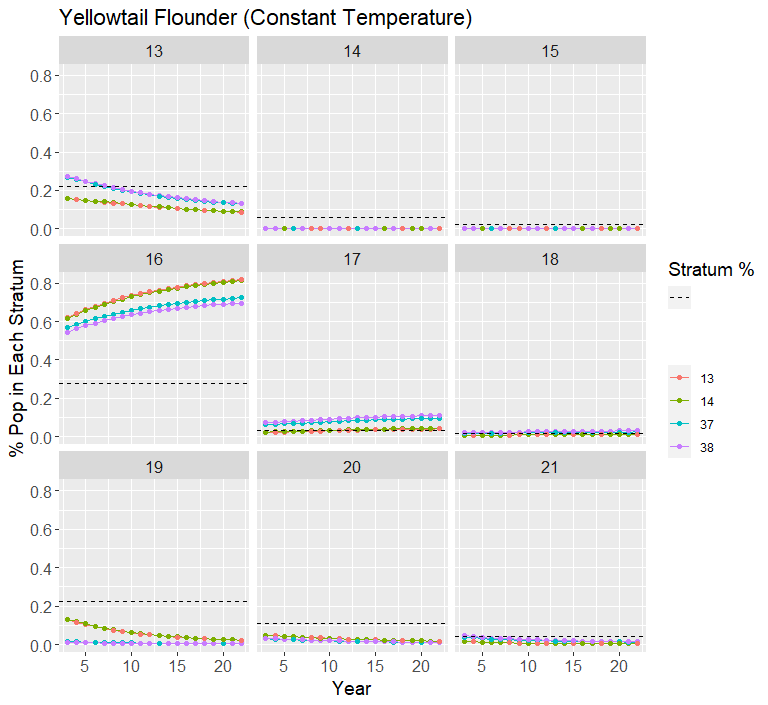
\includegraphics[width=0.475\linewidth]{Images/PercentPlots_ConPopConTemp_YT} 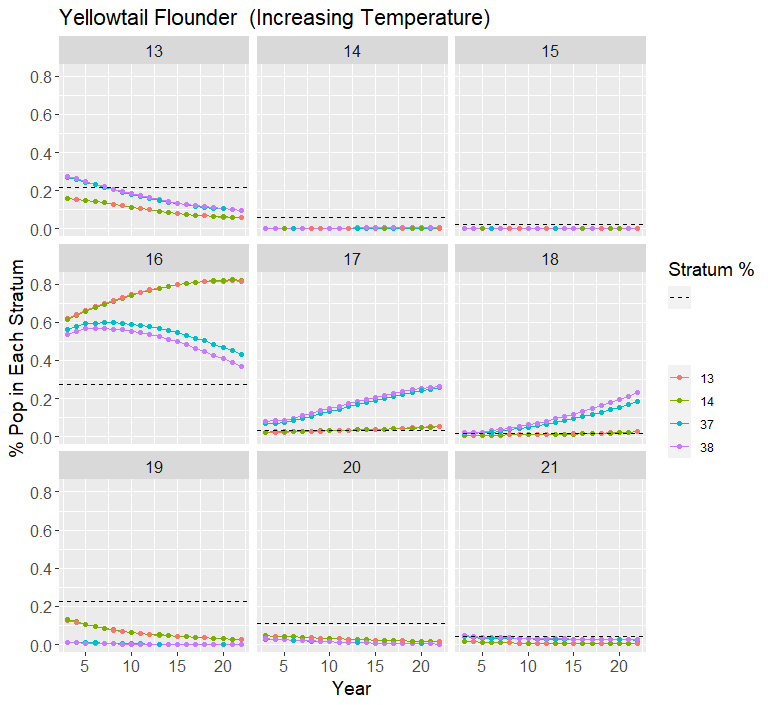
\includegraphics[width=0.475\linewidth]{Images/PercentPlots_ConPopIncTemp_YT} 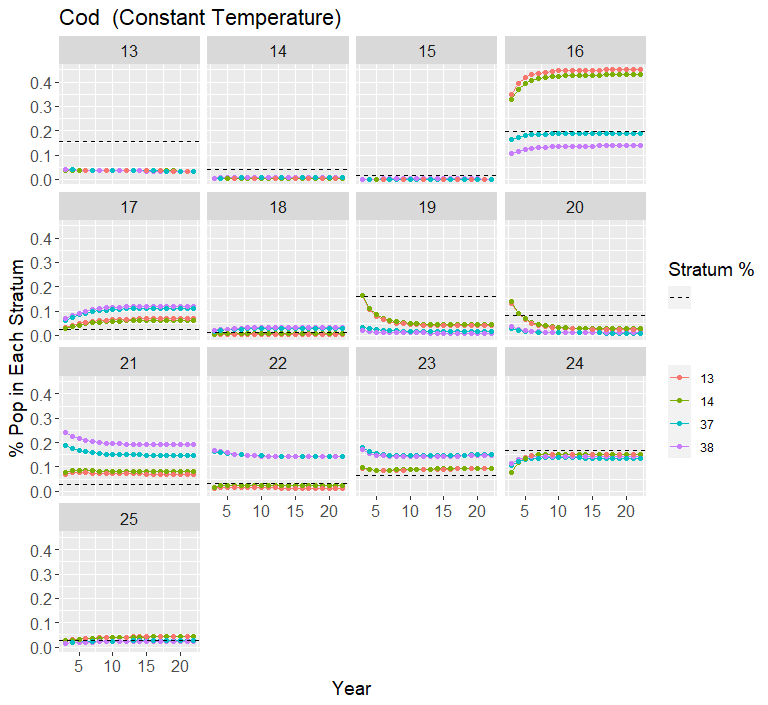
\includegraphics[width=0.475\linewidth]{Images/PercentPlots_DecPopConTemp_Cod} 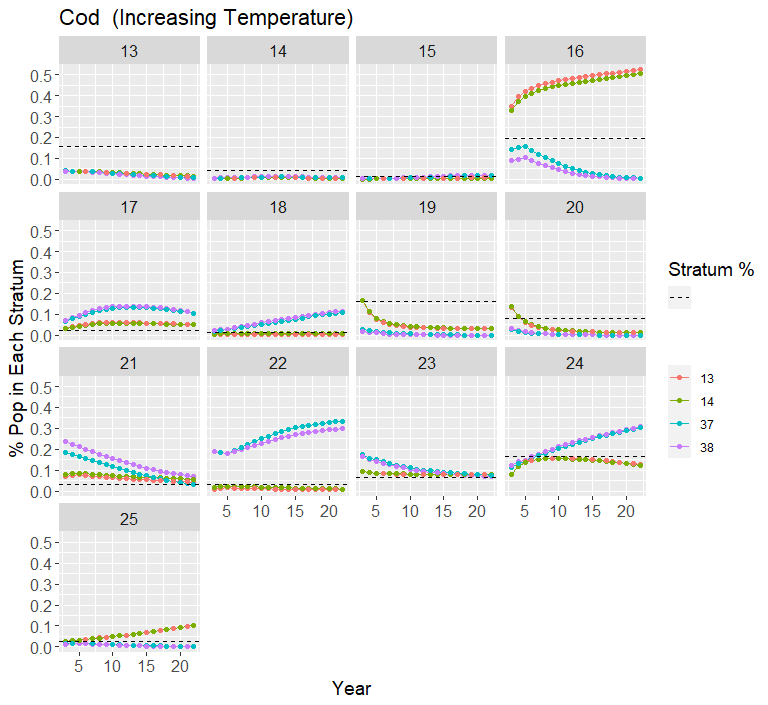
\includegraphics[width=0.475\linewidth]{Images/PercentPlots_DecPopIncTemp_Cod} 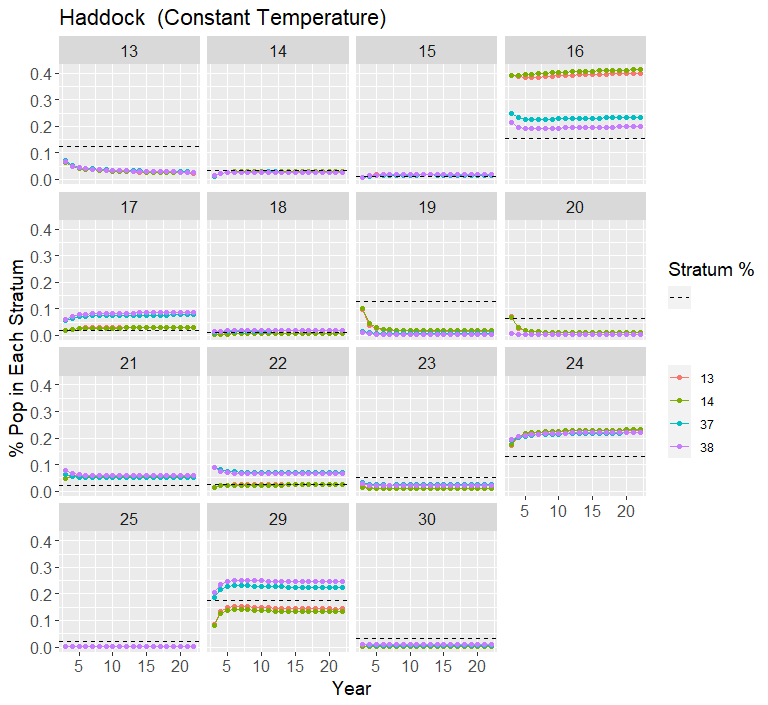
\includegraphics[width=0.475\linewidth]{Images/PercentPlots_IncPopConTemp_Had} 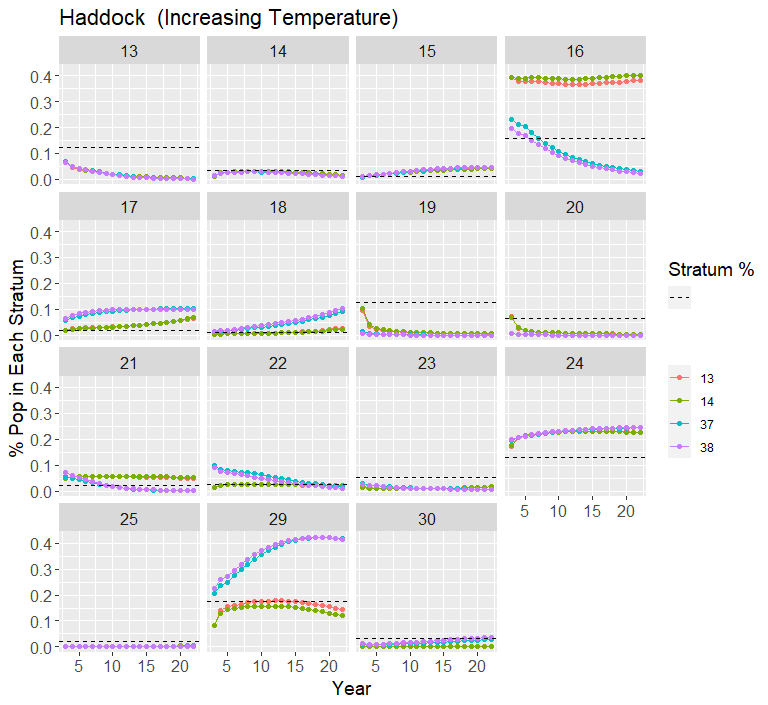
\includegraphics[width=0.475\linewidth]{Images/PercentPlots_IncPopIncTemp_Had} 

}

\caption{Percent of each species in each stratum for during survey weeks in our spatial simulations. All constant temperature scenarios follow the patterns on the left while increasing temperature scenarios follow the patterns on the right. See Figure 1 for a spatial reference of the Georges Bank strata.}\label{fig:PopPct}
\end{figure}

\begin{figure}

{\centering \includegraphics[width=0.9\linewidth]{Images/ratio_trend_YTF} \includegraphics[width=0.9\linewidth]{Images/ratio_trend_cod} \includegraphics[width=0.9\linewidth]{Images/ratio_trend_had} 

}

\caption{Representative example of typical ratio trend for each species, as shown on a log scale.}\label{fig:RatioTrend}
\end{figure}

\begin{figure}

{\centering \includegraphics[width=0.9\linewidth]{Images/Yellowtail_Estimate_Example} 

}

\caption{Representative example of biomass estimate trend for Yellowtail. Both scenarios have a relatively constant population with all strata being surveyed. The main difference is the left column has a repeating temperature gradient while the right column has increasing average temperature. }\label{fig:YTEstEx}
\end{figure}

\begin{figure}

{\centering \includegraphics[width=0.9\linewidth]{Images/Cod_Estimate_Example} 

}

\caption{Representative example of biomass estimate trend for Atlantic Cod. Both scenarios have a decreasing population trend with all strata being surveyed. The main difference is the left column has a repeating temperature gradient while the right column has increasing average temperature}\label{fig:CodEstEx}
\end{figure}

\begin{figure}

{\centering \includegraphics[width=0.9\linewidth]{Images/Haddock_Estimate_Example} 

}

\caption{Representative example of biomass estimate trend for Haddock. Both scenarios have an increasing population trend and a repeating temperature gradient. The main difference is the left column has all strata being surveyed while the right column has certain strata excluded from sampling}\label{fig:HadEstEx}
\end{figure}

\begin{figure}

{\centering \includegraphics[width=0.9\linewidth]{Images/covariate_plot3} 

}

\caption{Temperature covariate response plot and resulting population estimate for Haddock when the population was increasing over time, the average tempearture was increasing, and certain strata shown in Figure 1 were excluded from sampling.}\label{fig:CovResponse}
\end{figure}

\begin{table}

\caption{\label{tab:YTresultsallstrata}Yellowtail Flounder absolute error results with all strata included in calculations. Row colors correspond to the same settings applied in different seasons.}
\centering
\fontsize{10}{12}\selectfont
\begin{tabular}[t]{l|l|l|l|c|c|c}
\hline
\textbf{Temperature Scenario} & \textbf{Season} & \textbf{Covariate} & \textbf{Noise} & \textbf{VAST A} & \textbf{VAST B} & \textbf{Stratified Mean}\\
\hline
\multicolumn{1}{l}{\textbf{Constant Population}}\\
\hline
\cellcolor{black}{\textcolor{white}{\textbf{\hspace{1em}Constant}}} & \cellcolor{black}{\textcolor{white}{\textbf{spring}}} & \cellcolor{black}{\textcolor{white}{\textbf{no cov}}} & \cellcolor{black}{\textcolor{white}{\textbf{no}}} & \cellcolor{black}{\textcolor{white}{\textbf{0.13}}} & \cellcolor{black}{\textcolor{white}{\textbf{0.11}}} & \cellcolor{black}{\textcolor{white}{\textbf{0.21}}}\\
\hline
\cellcolor[HTML]{5C5E60}{\textcolor{white}{\textbf{\hspace{1em}Constant}}} & \cellcolor[HTML]{5C5E60}{\textcolor{white}{\textbf{spring}}} & \cellcolor[HTML]{5C5E60}{\textcolor{white}{\textbf{no cov}}} & \cellcolor[HTML]{5C5E60}{\textcolor{white}{\textbf{yes}}} & \cellcolor[HTML]{5C5E60}{\textcolor{white}{\textbf{0.14}}} & \cellcolor[HTML]{5C5E60}{\textcolor{white}{\textbf{0.16}}} & \cellcolor[HTML]{5C5E60}{\textcolor{white}{\textbf{0.25}}}\\
\hline
\cellcolor[HTML]{A4A4A4}{\textcolor{white}{\textbf{\hspace{1em}Constant}}} & \cellcolor[HTML]{A4A4A4}{\textcolor{white}{\textbf{spring}}} & \cellcolor[HTML]{A4A4A4}{\textcolor{white}{\textbf{w/ cov}}} & \cellcolor[HTML]{A4A4A4}{\textcolor{white}{\textbf{no}}} & \cellcolor[HTML]{A4A4A4}{\textcolor{white}{\textbf{0.07}}} & \cellcolor[HTML]{A4A4A4}{\textcolor{white}{\textbf{0.07}}} & \cellcolor[HTML]{A4A4A4}{\textcolor{white}{\textbf{n/a}}}\\
\hline
\cellcolor[HTML]{D2D2D2}{\textcolor{white}{\textbf{\hspace{1em}Constant}}} & \cellcolor[HTML]{D2D2D2}{\textcolor{white}{\textbf{spring}}} & \cellcolor[HTML]{D2D2D2}{\textcolor{white}{\textbf{w/ cov}}} & \cellcolor[HTML]{D2D2D2}{\textcolor{white}{\textbf{yes}}} & \cellcolor[HTML]{D2D2D2}{\textcolor{white}{\textbf{0.08}}} & \cellcolor[HTML]{D2D2D2}{\textcolor{white}{\textbf{0.08}}} & \cellcolor[HTML]{D2D2D2}{\textcolor{white}{\textbf{n/a}}}\\
\hline
\cellcolor{black}{\textcolor{white}{\textbf{\hspace{1em}Constant}}} & \cellcolor{black}{\textcolor{white}{\textbf{fall}}} & \cellcolor{black}{\textcolor{white}{\textbf{no cov}}} & \cellcolor{black}{\textcolor{white}{\textbf{no}}} & \cellcolor{black}{\textcolor{white}{\textbf{0.63}}} & \cellcolor{black}{\textcolor{white}{\textbf{0.68}}} & \cellcolor{black}{\textcolor{white}{\textbf{0.32}}}\\
\hline
\cellcolor[HTML]{5C5E60}{\textcolor{white}{\textbf{\hspace{1em}Constant}}} & \cellcolor[HTML]{5C5E60}{\textcolor{white}{\textbf{fall}}} & \cellcolor[HTML]{5C5E60}{\textcolor{white}{\textbf{no cov}}} & \cellcolor[HTML]{5C5E60}{\textcolor{white}{\textbf{yes}}} & \cellcolor[HTML]{5C5E60}{\textcolor{white}{\textbf{0.80}}} & \cellcolor[HTML]{5C5E60}{\textcolor{white}{\textbf{0.77}}} & \cellcolor[HTML]{5C5E60}{\textcolor{white}{\textbf{0.31}}}\\
\hline
\cellcolor[HTML]{A4A4A4}{\textcolor{white}{\textbf{\hspace{1em}Constant}}} & \cellcolor[HTML]{A4A4A4}{\textcolor{white}{\textbf{fall}}} & \cellcolor[HTML]{A4A4A4}{\textcolor{white}{\textbf{w/ cov}}} & \cellcolor[HTML]{A4A4A4}{\textcolor{white}{\textbf{no}}} & \cellcolor[HTML]{A4A4A4}{\textcolor{white}{\textbf{0.14}}} & \cellcolor[HTML]{A4A4A4}{\textcolor{white}{\textbf{0.08}}} & \cellcolor[HTML]{A4A4A4}{\textcolor{white}{\textbf{n/a}}}\\
\hline
\cellcolor[HTML]{D2D2D2}{\textcolor{white}{\textbf{\hspace{1em}Constant}}} & \cellcolor[HTML]{D2D2D2}{\textcolor{white}{\textbf{fall}}} & \cellcolor[HTML]{D2D2D2}{\textcolor{white}{\textbf{w/ cov}}} & \cellcolor[HTML]{D2D2D2}{\textcolor{white}{\textbf{yes}}} & \cellcolor[HTML]{D2D2D2}{\textcolor{white}{\textbf{0.17}}} & \cellcolor[HTML]{D2D2D2}{\textcolor{white}{\textbf{0.11}}} & \cellcolor[HTML]{D2D2D2}{\textcolor{white}{\textbf{n/a}}}\\
\hline
\cellcolor{black}{\textcolor{white}{\textbf{\hspace{1em}Increasing}}} & \cellcolor{black}{\textcolor{white}{\textbf{spring}}} & \cellcolor{black}{\textcolor{white}{\textbf{no cov}}} & \cellcolor{black}{\textcolor{white}{\textbf{no}}} & \cellcolor{black}{\textcolor{white}{\textbf{0.14}}} & \cellcolor{black}{\textcolor{white}{\textbf{0.11}}} & \cellcolor{black}{\textcolor{white}{\textbf{0.28}}}\\
\hline
\cellcolor[HTML]{5C5E60}{\textcolor{white}{\textbf{\hspace{1em}Increasing}}} & \cellcolor[HTML]{5C5E60}{\textcolor{white}{\textbf{spring}}} & \cellcolor[HTML]{5C5E60}{\textcolor{white}{\textbf{no cov}}} & \cellcolor[HTML]{5C5E60}{\textcolor{white}{\textbf{yes}}} & \cellcolor[HTML]{5C5E60}{\textcolor{white}{\textbf{0.18}}} & \cellcolor[HTML]{5C5E60}{\textcolor{white}{\textbf{0.15}}} & \cellcolor[HTML]{5C5E60}{\textcolor{white}{\textbf{0.28}}}\\
\hline
\cellcolor[HTML]{A4A4A4}{\textcolor{white}{\textbf{\hspace{1em}Increasing}}} & \cellcolor[HTML]{A4A4A4}{\textcolor{white}{\textbf{spring}}} & \cellcolor[HTML]{A4A4A4}{\textcolor{white}{\textbf{w/ cov}}} & \cellcolor[HTML]{A4A4A4}{\textcolor{white}{\textbf{no}}} & \cellcolor[HTML]{A4A4A4}{\textcolor{white}{\textbf{0.05}}} & \cellcolor[HTML]{A4A4A4}{\textcolor{white}{\textbf{0.06}}} & \cellcolor[HTML]{A4A4A4}{\textcolor{white}{\textbf{n/a}}}\\
\hline
\cellcolor[HTML]{D2D2D2}{\textcolor{white}{\textbf{\hspace{1em}Increasing}}} & \cellcolor[HTML]{D2D2D2}{\textcolor{white}{\textbf{spring}}} & \cellcolor[HTML]{D2D2D2}{\textcolor{white}{\textbf{w/ cov}}} & \cellcolor[HTML]{D2D2D2}{\textcolor{white}{\textbf{yes}}} & \cellcolor[HTML]{D2D2D2}{\textcolor{white}{\textbf{0.10}}} & \cellcolor[HTML]{D2D2D2}{\textcolor{white}{\textbf{0.12}}} & \cellcolor[HTML]{D2D2D2}{\textcolor{white}{\textbf{n/a}}}\\
\hline
\cellcolor{black}{\textcolor{white}{\textbf{\hspace{1em}Increasing}}} & \cellcolor{black}{\textcolor{white}{\textbf{fall}}} & \cellcolor{black}{\textcolor{white}{\textbf{no cov}}} & \cellcolor{black}{\textcolor{white}{\textbf{no}}} & \cellcolor{black}{\textcolor{white}{\textbf{1.46}}} & \cellcolor{black}{\textcolor{white}{\textbf{1.26}}} & \cellcolor{black}{\textcolor{white}{\textbf{0.51}}}\\
\hline
\cellcolor[HTML]{5C5E60}{\textcolor{white}{\textbf{\hspace{1em}Increasing}}} & \cellcolor[HTML]{5C5E60}{\textcolor{white}{\textbf{fall}}} & \cellcolor[HTML]{5C5E60}{\textcolor{white}{\textbf{no cov}}} & \cellcolor[HTML]{5C5E60}{\textcolor{white}{\textbf{yes}}} & \cellcolor[HTML]{5C5E60}{\textcolor{white}{\textbf{1.40}}} & \cellcolor[HTML]{5C5E60}{\textcolor{white}{\textbf{1.38}}} & \cellcolor[HTML]{5C5E60}{\textcolor{white}{\textbf{0.5}}}\\
\hline
\cellcolor[HTML]{A4A4A4}{\textcolor{white}{\textbf{\hspace{1em}Increasing}}} & \cellcolor[HTML]{A4A4A4}{\textcolor{white}{\textbf{fall}}} & \cellcolor[HTML]{A4A4A4}{\textcolor{white}{\textbf{w/ cov}}} & \cellcolor[HTML]{A4A4A4}{\textcolor{white}{\textbf{no}}} & \cellcolor[HTML]{A4A4A4}{\textcolor{white}{\textbf{0.21}}} & \cellcolor[HTML]{A4A4A4}{\textcolor{white}{\textbf{0.23}}} & \cellcolor[HTML]{A4A4A4}{\textcolor{white}{\textbf{n/a}}}\\
\hline
\cellcolor[HTML]{D2D2D2}{\textcolor{white}{\textbf{\hspace{1em}Increasing}}} & \cellcolor[HTML]{D2D2D2}{\textcolor{white}{\textbf{fall}}} & \cellcolor[HTML]{D2D2D2}{\textcolor{white}{\textbf{w/ cov}}} & \cellcolor[HTML]{D2D2D2}{\textcolor{white}{\textbf{yes}}} & \cellcolor[HTML]{D2D2D2}{\textcolor{white}{\textbf{0.30}}} & \cellcolor[HTML]{D2D2D2}{\textcolor{white}{\textbf{0.28}}} & \cellcolor[HTML]{D2D2D2}{\textcolor{white}{\textbf{n/a}}}\\
\hline
\multicolumn{1}{l}{\textbf{Decreasing Population}}\\
\hline
\cellcolor{black}{\textcolor{white}{\textbf{\hspace{1em}Constant}}} & \cellcolor{black}{\textcolor{white}{\textbf{spring}}} & \cellcolor{black}{\textcolor{white}{\textbf{no cov}}} & \cellcolor{black}{\textcolor{white}{\textbf{no}}} & \cellcolor{black}{\textcolor{white}{\textbf{0.11}}} & \cellcolor{black}{\textcolor{white}{\textbf{0.08}}} & \cellcolor{black}{\textcolor{white}{\textbf{0.23}}}\\
\hline
\cellcolor[HTML]{5C5E60}{\textcolor{white}{\textbf{\hspace{1em}Constant}}} & \cellcolor[HTML]{5C5E60}{\textcolor{white}{\textbf{spring}}} & \cellcolor[HTML]{5C5E60}{\textcolor{white}{\textbf{no cov}}} & \cellcolor[HTML]{5C5E60}{\textcolor{white}{\textbf{yes}}} & \cellcolor[HTML]{5C5E60}{\textcolor{white}{\textbf{0.12}}} & \cellcolor[HTML]{5C5E60}{\textcolor{white}{\textbf{0.11}}} & \cellcolor[HTML]{5C5E60}{\textcolor{white}{\textbf{0.27}}}\\
\hline
\cellcolor[HTML]{A4A4A4}{\textcolor{white}{\textbf{\hspace{1em}Constant}}} & \cellcolor[HTML]{A4A4A4}{\textcolor{white}{\textbf{spring}}} & \cellcolor[HTML]{A4A4A4}{\textcolor{white}{\textbf{w/ cov}}} & \cellcolor[HTML]{A4A4A4}{\textcolor{white}{\textbf{no}}} & \cellcolor[HTML]{A4A4A4}{\textcolor{white}{\textbf{0.07}}} & \cellcolor[HTML]{A4A4A4}{\textcolor{white}{\textbf{0.06}}} & \cellcolor[HTML]{A4A4A4}{\textcolor{white}{\textbf{n/a}}}\\
\hline
\cellcolor[HTML]{D2D2D2}{\textcolor{white}{\textbf{\hspace{1em}Constant}}} & \cellcolor[HTML]{D2D2D2}{\textcolor{white}{\textbf{spring}}} & \cellcolor[HTML]{D2D2D2}{\textcolor{white}{\textbf{w/ cov}}} & \cellcolor[HTML]{D2D2D2}{\textcolor{white}{\textbf{yes}}} & \cellcolor[HTML]{D2D2D2}{\textcolor{white}{\textbf{0.11}}} & \cellcolor[HTML]{D2D2D2}{\textcolor{white}{\textbf{0.07}}} & \cellcolor[HTML]{D2D2D2}{\textcolor{white}{\textbf{n/a}}}\\
\hline
\cellcolor{black}{\textcolor{white}{\textbf{\hspace{1em}Constant}}} & \cellcolor{black}{\textcolor{white}{\textbf{fall}}} & \cellcolor{black}{\textcolor{white}{\textbf{no cov}}} & \cellcolor{black}{\textcolor{white}{\textbf{no}}} & \cellcolor{black}{\textcolor{white}{\textbf{0.97}}} & \cellcolor{black}{\textcolor{white}{\textbf{0.81}}} & \cellcolor{black}{\textcolor{white}{\textbf{0.41}}}\\
\hline
\cellcolor[HTML]{5C5E60}{\textcolor{white}{\textbf{\hspace{1em}Constant}}} & \cellcolor[HTML]{5C5E60}{\textcolor{white}{\textbf{fall}}} & \cellcolor[HTML]{5C5E60}{\textcolor{white}{\textbf{no cov}}} & \cellcolor[HTML]{5C5E60}{\textcolor{white}{\textbf{yes}}} & \cellcolor[HTML]{5C5E60}{\textcolor{white}{\textbf{0.99}}} & \cellcolor[HTML]{5C5E60}{\textcolor{white}{\textbf{1.09}}} & \cellcolor[HTML]{5C5E60}{\textcolor{white}{\textbf{0.37}}}\\
\hline
\cellcolor[HTML]{A4A4A4}{\textcolor{white}{\textbf{\hspace{1em}Constant}}} & \cellcolor[HTML]{A4A4A4}{\textcolor{white}{\textbf{fall}}} & \cellcolor[HTML]{A4A4A4}{\textcolor{white}{\textbf{w/ cov}}} & \cellcolor[HTML]{A4A4A4}{\textcolor{white}{\textbf{no}}} & \cellcolor[HTML]{A4A4A4}{\textcolor{white}{\textbf{0.16}}} & \cellcolor[HTML]{A4A4A4}{\textcolor{white}{\textbf{0.08}}} & \cellcolor[HTML]{A4A4A4}{\textcolor{white}{\textbf{n/a}}}\\
\hline
\cellcolor[HTML]{D2D2D2}{\textcolor{white}{\textbf{\hspace{1em}Constant}}} & \cellcolor[HTML]{D2D2D2}{\textcolor{white}{\textbf{fall}}} & \cellcolor[HTML]{D2D2D2}{\textcolor{white}{\textbf{w/ cov}}} & \cellcolor[HTML]{D2D2D2}{\textcolor{white}{\textbf{yes}}} & \cellcolor[HTML]{D2D2D2}{\textcolor{white}{\textbf{0.29}}} & \cellcolor[HTML]{D2D2D2}{\textcolor{white}{\textbf{0.18}}} & \cellcolor[HTML]{D2D2D2}{\textcolor{white}{\textbf{n/a}}}\\
\hline
\cellcolor{black}{\textcolor{white}{\textbf{\hspace{1em}Increasing}}} & \cellcolor{black}{\textcolor{white}{\textbf{spring}}} & \cellcolor{black}{\textcolor{white}{\textbf{no cov}}} & \cellcolor{black}{\textcolor{white}{\textbf{no}}} & \cellcolor{black}{\textcolor{white}{\textbf{0.17}}} & \cellcolor{black}{\textcolor{white}{\textbf{0.15}}} & \cellcolor{black}{\textcolor{white}{\textbf{0.22}}}\\
\hline
\cellcolor[HTML]{5C5E60}{\textcolor{white}{\textbf{\hspace{1em}Increasing}}} & \cellcolor[HTML]{5C5E60}{\textcolor{white}{\textbf{spring}}} & \cellcolor[HTML]{5C5E60}{\textcolor{white}{\textbf{no cov}}} & \cellcolor[HTML]{5C5E60}{\textcolor{white}{\textbf{yes}}} & \cellcolor[HTML]{5C5E60}{\textcolor{white}{\textbf{0.15}}} & \cellcolor[HTML]{5C5E60}{\textcolor{white}{\textbf{0.17}}} & \cellcolor[HTML]{5C5E60}{\textcolor{white}{\textbf{0.26}}}\\
\hline
\cellcolor[HTML]{A4A4A4}{\textcolor{white}{\textbf{\hspace{1em}Increasing}}} & \cellcolor[HTML]{A4A4A4}{\textcolor{white}{\textbf{spring}}} & \cellcolor[HTML]{A4A4A4}{\textcolor{white}{\textbf{w/ cov}}} & \cellcolor[HTML]{A4A4A4}{\textcolor{white}{\textbf{no}}} & \cellcolor[HTML]{A4A4A4}{\textcolor{white}{\textbf{0.08}}} & \cellcolor[HTML]{A4A4A4}{\textcolor{white}{\textbf{0.07}}} & \cellcolor[HTML]{A4A4A4}{\textcolor{white}{\textbf{n/a}}}\\
\hline
\cellcolor[HTML]{D2D2D2}{\textcolor{white}{\textbf{\hspace{1em}Increasing}}} & \cellcolor[HTML]{D2D2D2}{\textcolor{white}{\textbf{spring}}} & \cellcolor[HTML]{D2D2D2}{\textcolor{white}{\textbf{w/ cov}}} & \cellcolor[HTML]{D2D2D2}{\textcolor{white}{\textbf{yes}}} & \cellcolor[HTML]{D2D2D2}{\textcolor{white}{\textbf{0.16}}} & \cellcolor[HTML]{D2D2D2}{\textcolor{white}{\textbf{0.10}}} & \cellcolor[HTML]{D2D2D2}{\textcolor{white}{\textbf{n/a}}}\\
\hline
\cellcolor{black}{\textcolor{white}{\textbf{\hspace{1em}Increasing}}} & \cellcolor{black}{\textcolor{white}{\textbf{fall}}} & \cellcolor{black}{\textcolor{white}{\textbf{no cov}}} & \cellcolor{black}{\textcolor{white}{\textbf{no}}} & \cellcolor{black}{\textcolor{white}{\textbf{1.17}}} & \cellcolor{black}{\textcolor{white}{\textbf{1.06}}} & \cellcolor{black}{\textcolor{white}{\textbf{0.28}}}\\
\hline
\cellcolor[HTML]{5C5E60}{\textcolor{white}{\textbf{\hspace{1em}Increasing}}} & \cellcolor[HTML]{5C5E60}{\textcolor{white}{\textbf{fall}}} & \cellcolor[HTML]{5C5E60}{\textcolor{white}{\textbf{no cov}}} & \cellcolor[HTML]{5C5E60}{\textcolor{white}{\textbf{yes}}} & \cellcolor[HTML]{5C5E60}{\textcolor{white}{\textbf{1.14}}} & \cellcolor[HTML]{5C5E60}{\textcolor{white}{\textbf{1.10}}} & \cellcolor[HTML]{5C5E60}{\textcolor{white}{\textbf{0.25}}}\\
\hline
\cellcolor[HTML]{A4A4A4}{\textcolor{white}{\textbf{\hspace{1em}Increasing}}} & \cellcolor[HTML]{A4A4A4}{\textcolor{white}{\textbf{fall}}} & \cellcolor[HTML]{A4A4A4}{\textcolor{white}{\textbf{w/ cov}}} & \cellcolor[HTML]{A4A4A4}{\textcolor{white}{\textbf{no}}} & \cellcolor[HTML]{A4A4A4}{\textcolor{white}{\textbf{0.40}}} & \cellcolor[HTML]{A4A4A4}{\textcolor{white}{\textbf{0.15}}} & \cellcolor[HTML]{A4A4A4}{\textcolor{white}{\textbf{n/a}}}\\
\hline
\cellcolor[HTML]{D2D2D2}{\textcolor{white}{\textbf{\hspace{1em}Increasing}}} & \cellcolor[HTML]{D2D2D2}{\textcolor{white}{\textbf{fall}}} & \cellcolor[HTML]{D2D2D2}{\textcolor{white}{\textbf{w/ cov}}} & \cellcolor[HTML]{D2D2D2}{\textcolor{white}{\textbf{yes}}} & \cellcolor[HTML]{D2D2D2}{\textcolor{white}{\textbf{0.40}}} & \cellcolor[HTML]{D2D2D2}{\textcolor{white}{\textbf{0.20}}} & \cellcolor[HTML]{D2D2D2}{\textcolor{white}{\textbf{n/a}}}\\
\hline
\multicolumn{1}{l}{\textbf{Increasing Population}}\\
\hline
\cellcolor{black}{\textcolor{white}{\textbf{\hspace{1em}Constant}}} & \cellcolor{black}{\textcolor{white}{\textbf{spring}}} & \cellcolor{black}{\textcolor{white}{\textbf{no cov}}} & \cellcolor{black}{\textcolor{white}{\textbf{no}}} & \cellcolor{black}{\textcolor{white}{\textbf{0.46}}} & \cellcolor{black}{\textcolor{white}{\textbf{0.13}}} & \cellcolor{black}{\textcolor{white}{\textbf{0.16}}}\\
\hline
\cellcolor[HTML]{5C5E60}{\textcolor{white}{\textbf{\hspace{1em}Constant}}} & \cellcolor[HTML]{5C5E60}{\textcolor{white}{\textbf{spring}}} & \cellcolor[HTML]{5C5E60}{\textcolor{white}{\textbf{no cov}}} & \cellcolor[HTML]{5C5E60}{\textcolor{white}{\textbf{yes}}} & \cellcolor[HTML]{5C5E60}{\textcolor{white}{\textbf{0.43}}} & \cellcolor[HTML]{5C5E60}{\textcolor{white}{\textbf{0.21}}} & \cellcolor[HTML]{5C5E60}{\textcolor{white}{\textbf{0.22}}}\\
\hline
\cellcolor[HTML]{A4A4A4}{\textcolor{white}{\textbf{\hspace{1em}Constant}}} & \cellcolor[HTML]{A4A4A4}{\textcolor{white}{\textbf{spring}}} & \cellcolor[HTML]{A4A4A4}{\textcolor{white}{\textbf{w/ cov}}} & \cellcolor[HTML]{A4A4A4}{\textcolor{white}{\textbf{no}}} & \cellcolor[HTML]{A4A4A4}{\textcolor{white}{\textbf{0.06}}} & \cellcolor[HTML]{A4A4A4}{\textcolor{white}{\textbf{0.06}}} & \cellcolor[HTML]{A4A4A4}{\textcolor{white}{\textbf{n/a}}}\\
\hline
\cellcolor[HTML]{D2D2D2}{\textcolor{white}{\textbf{\hspace{1em}Constant}}} & \cellcolor[HTML]{D2D2D2}{\textcolor{white}{\textbf{spring}}} & \cellcolor[HTML]{D2D2D2}{\textcolor{white}{\textbf{w/ cov}}} & \cellcolor[HTML]{D2D2D2}{\textcolor{white}{\textbf{yes}}} & \cellcolor[HTML]{D2D2D2}{\textcolor{white}{\textbf{0.08}}} & \cellcolor[HTML]{D2D2D2}{\textcolor{white}{\textbf{0.07}}} & \cellcolor[HTML]{D2D2D2}{\textcolor{white}{\textbf{n/a}}}\\
\hline
\cellcolor{black}{\textcolor{white}{\textbf{\hspace{1em}Constant}}} & \cellcolor{black}{\textcolor{white}{\textbf{fall}}} & \cellcolor{black}{\textcolor{white}{\textbf{no cov}}} & \cellcolor{black}{\textcolor{white}{\textbf{no}}} & \cellcolor{black}{\textcolor{white}{\textbf{0.40}}} & \cellcolor{black}{\textcolor{white}{\textbf{0.36}}} & \cellcolor{black}{\textcolor{white}{\textbf{0.34}}}\\
\hline
\cellcolor[HTML]{5C5E60}{\textcolor{white}{\textbf{\hspace{1em}Constant}}} & \cellcolor[HTML]{5C5E60}{\textcolor{white}{\textbf{fall}}} & \cellcolor[HTML]{5C5E60}{\textcolor{white}{\textbf{no cov}}} & \cellcolor[HTML]{5C5E60}{\textcolor{white}{\textbf{yes}}} & \cellcolor[HTML]{5C5E60}{\textcolor{white}{\textbf{0.38}}} & \cellcolor[HTML]{5C5E60}{\textcolor{white}{\textbf{0.44}}} & \cellcolor[HTML]{5C5E60}{\textcolor{white}{\textbf{0.46}}}\\
\hline
\cellcolor[HTML]{A4A4A4}{\textcolor{white}{\textbf{\hspace{1em}Constant}}} & \cellcolor[HTML]{A4A4A4}{\textcolor{white}{\textbf{fall}}} & \cellcolor[HTML]{A4A4A4}{\textcolor{white}{\textbf{w/ cov}}} & \cellcolor[HTML]{A4A4A4}{\textcolor{white}{\textbf{no}}} & \cellcolor[HTML]{A4A4A4}{\textcolor{white}{\textbf{0.11}}} & \cellcolor[HTML]{A4A4A4}{\textcolor{white}{\textbf{0.08}}} & \cellcolor[HTML]{A4A4A4}{\textcolor{white}{\textbf{n/a}}}\\
\hline
\cellcolor[HTML]{D2D2D2}{\textcolor{white}{\textbf{\hspace{1em}Constant}}} & \cellcolor[HTML]{D2D2D2}{\textcolor{white}{\textbf{fall}}} & \cellcolor[HTML]{D2D2D2}{\textcolor{white}{\textbf{w/ cov}}} & \cellcolor[HTML]{D2D2D2}{\textcolor{white}{\textbf{yes}}} & \cellcolor[HTML]{D2D2D2}{\textcolor{white}{\textbf{0.24}}} & \cellcolor[HTML]{D2D2D2}{\textcolor{white}{\textbf{0.17}}} & \cellcolor[HTML]{D2D2D2}{\textcolor{white}{\textbf{n/a}}}\\
\hline
\cellcolor{black}{\textcolor{white}{\textbf{\hspace{1em}Increasing}}} & \cellcolor{black}{\textcolor{white}{\textbf{spring}}} & \cellcolor{black}{\textcolor{white}{\textbf{no cov}}} & \cellcolor{black}{\textcolor{white}{\textbf{no}}} & \cellcolor{black}{\textcolor{white}{\textbf{0.16}}} & \cellcolor{black}{\textcolor{white}{\textbf{0.13}}} & \cellcolor{black}{\textcolor{white}{\textbf{0.32}}}\\
\hline
\cellcolor[HTML]{5C5E60}{\textcolor{white}{\textbf{\hspace{1em}Increasing}}} & \cellcolor[HTML]{5C5E60}{\textcolor{white}{\textbf{spring}}} & \cellcolor[HTML]{5C5E60}{\textcolor{white}{\textbf{no cov}}} & \cellcolor[HTML]{5C5E60}{\textcolor{white}{\textbf{yes}}} & \cellcolor[HTML]{5C5E60}{\textcolor{white}{\textbf{0.21}}} & \cellcolor[HTML]{5C5E60}{\textcolor{white}{\textbf{0.16}}} & \cellcolor[HTML]{5C5E60}{\textcolor{white}{\textbf{0.32}}}\\
\hline
\cellcolor[HTML]{A4A4A4}{\textcolor{white}{\textbf{\hspace{1em}Increasing}}} & \cellcolor[HTML]{A4A4A4}{\textcolor{white}{\textbf{spring}}} & \cellcolor[HTML]{A4A4A4}{\textcolor{white}{\textbf{w/ cov}}} & \cellcolor[HTML]{A4A4A4}{\textcolor{white}{\textbf{no}}} & \cellcolor[HTML]{A4A4A4}{\textcolor{white}{\textbf{0.06}}} & \cellcolor[HTML]{A4A4A4}{\textcolor{white}{\textbf{0.07}}} & \cellcolor[HTML]{A4A4A4}{\textcolor{white}{\textbf{n/a}}}\\
\hline
\cellcolor[HTML]{D2D2D2}{\textcolor{white}{\textbf{\hspace{1em}Increasing}}} & \cellcolor[HTML]{D2D2D2}{\textcolor{white}{\textbf{spring}}} & \cellcolor[HTML]{D2D2D2}{\textcolor{white}{\textbf{w/ cov}}} & \cellcolor[HTML]{D2D2D2}{\textcolor{white}{\textbf{yes}}} & \cellcolor[HTML]{D2D2D2}{\textcolor{white}{\textbf{0.12}}} & \cellcolor[HTML]{D2D2D2}{\textcolor{white}{\textbf{0.10}}} & \cellcolor[HTML]{D2D2D2}{\textcolor{white}{\textbf{n/a}}}\\
\hline
\cellcolor{black}{\textcolor{white}{\textbf{\hspace{1em}Increasing}}} & \cellcolor{black}{\textcolor{white}{\textbf{fall}}} & \cellcolor{black}{\textcolor{white}{\textbf{no cov}}} & \cellcolor{black}{\textcolor{white}{\textbf{no}}} & \cellcolor{black}{\textcolor{white}{\textbf{0.71}}} & \cellcolor{black}{\textcolor{white}{\textbf{0.66}}} & \cellcolor{black}{\textcolor{white}{\textbf{0.3}}}\\
\hline
\cellcolor[HTML]{5C5E60}{\textcolor{white}{\textbf{\hspace{1em}Increasing}}} & \cellcolor[HTML]{5C5E60}{\textcolor{white}{\textbf{fall}}} & \cellcolor[HTML]{5C5E60}{\textcolor{white}{\textbf{no cov}}} & \cellcolor[HTML]{5C5E60}{\textcolor{white}{\textbf{yes}}} & \cellcolor[HTML]{5C5E60}{\textcolor{white}{\textbf{1.03}}} & \cellcolor[HTML]{5C5E60}{\textcolor{white}{\textbf{0.71}}} & \cellcolor[HTML]{5C5E60}{\textcolor{white}{\textbf{0.39}}}\\
\hline
\cellcolor[HTML]{A4A4A4}{\textcolor{white}{\textbf{\hspace{1em}Increasing}}} & \cellcolor[HTML]{A4A4A4}{\textcolor{white}{\textbf{fall}}} & \cellcolor[HTML]{A4A4A4}{\textcolor{white}{\textbf{w/ cov}}} & \cellcolor[HTML]{A4A4A4}{\textcolor{white}{\textbf{no}}} & \cellcolor[HTML]{A4A4A4}{\textcolor{white}{\textbf{0.43}}} & \cellcolor[HTML]{A4A4A4}{\textcolor{white}{\textbf{0.21}}} & \cellcolor[HTML]{A4A4A4}{\textcolor{white}{\textbf{n/a}}}\\
\hline
\cellcolor[HTML]{D2D2D2}{\textcolor{white}{\textbf{\hspace{1em}Increasing}}} & \cellcolor[HTML]{D2D2D2}{\textcolor{white}{\textbf{fall}}} & \cellcolor[HTML]{D2D2D2}{\textcolor{white}{\textbf{w/ cov}}} & \cellcolor[HTML]{D2D2D2}{\textcolor{white}{\textbf{yes}}} & \cellcolor[HTML]{D2D2D2}{\textcolor{white}{\textbf{0.51}}} & \cellcolor[HTML]{D2D2D2}{\textcolor{white}{\textbf{0.37}}} & \cellcolor[HTML]{D2D2D2}{\textcolor{white}{\textbf{n/a}}}\\
\hline
\end{tabular}
\end{table}
\begin{table}

\caption{\label{tab:YTresultsreducedstrata}Yellowtail Flounder absoloute error results with certain strata excluded from calculations. Row colors correspond to the same settings applied in different seasons.}
\centering
\fontsize{10}{12}\selectfont
\begin{tabular}[t]{l|l|l|l|c|c|c}
\hline
\textbf{Temperature Scenario} & \textbf{Season} & \textbf{Covariate} & \textbf{Noise} & \textbf{VAST A} & \textbf{VAST B} & \textbf{Stratified Mean}\\
\hline
\multicolumn{1}{l}{\textbf{Constant Population}}\\
\hline
\cellcolor{black}{\textcolor{white}{\textbf{\hspace{1em}Constant}}} & \cellcolor{black}{\textcolor{white}{\textbf{spring}}} & \cellcolor{black}{\textcolor{white}{\textbf{no cov}}} & \cellcolor{black}{\textcolor{white}{\textbf{no}}} & \cellcolor{black}{\textcolor{white}{\textbf{0.24}}} & \cellcolor{black}{\textcolor{white}{\textbf{0.19}}} & \cellcolor{black}{\textcolor{white}{\textbf{0.27}}}\\
\hline
\cellcolor[HTML]{5C5E60}{\textcolor{white}{\textbf{\hspace{1em}Constant}}} & \cellcolor[HTML]{5C5E60}{\textcolor{white}{\textbf{spring}}} & \cellcolor[HTML]{5C5E60}{\textcolor{white}{\textbf{no cov}}} & \cellcolor[HTML]{5C5E60}{\textcolor{white}{\textbf{yes}}} & \cellcolor[HTML]{5C5E60}{\textcolor{white}{\textbf{0.16}}} & \cellcolor[HTML]{5C5E60}{\textcolor{white}{\textbf{0.15}}} & \cellcolor[HTML]{5C5E60}{\textcolor{white}{\textbf{0.22}}}\\
\hline
\cellcolor[HTML]{A4A4A4}{\textcolor{white}{\textbf{\hspace{1em}Constant}}} & \cellcolor[HTML]{A4A4A4}{\textcolor{white}{\textbf{spring}}} & \cellcolor[HTML]{A4A4A4}{\textcolor{white}{\textbf{w/ cov}}} & \cellcolor[HTML]{A4A4A4}{\textcolor{white}{\textbf{no}}} & \cellcolor[HTML]{A4A4A4}{\textcolor{white}{\textbf{0.19}}} & \cellcolor[HTML]{A4A4A4}{\textcolor{white}{\textbf{0.19}}} & \cellcolor[HTML]{A4A4A4}{\textcolor{white}{\textbf{\vphantom{1} n/a}}}\\
\hline
\cellcolor[HTML]{D2D2D2}{\textcolor{white}{\textbf{\hspace{1em}Constant}}} & \cellcolor[HTML]{D2D2D2}{\textcolor{white}{\textbf{spring}}} & \cellcolor[HTML]{D2D2D2}{\textcolor{white}{\textbf{w/ cov}}} & \cellcolor[HTML]{D2D2D2}{\textcolor{white}{\textbf{yes}}} & \cellcolor[HTML]{D2D2D2}{\textcolor{white}{\textbf{0.12}}} & \cellcolor[HTML]{D2D2D2}{\textcolor{white}{\textbf{0.14}}} & \cellcolor[HTML]{D2D2D2}{\textcolor{white}{\textbf{n/a}}}\\
\hline
\cellcolor{black}{\textcolor{white}{\textbf{\hspace{1em}Constant}}} & \cellcolor{black}{\textcolor{white}{\textbf{fall}}} & \cellcolor{black}{\textcolor{white}{\textbf{no cov}}} & \cellcolor{black}{\textcolor{white}{\textbf{no}}} & \cellcolor{black}{\textcolor{white}{\textbf{0.30}}} & \cellcolor{black}{\textcolor{white}{\textbf{0.25}}} & \cellcolor{black}{\textcolor{white}{\textbf{0.47}}}\\
\hline
\cellcolor[HTML]{5C5E60}{\textcolor{white}{\textbf{\hspace{1em}Constant}}} & \cellcolor[HTML]{5C5E60}{\textcolor{white}{\textbf{fall}}} & \cellcolor[HTML]{5C5E60}{\textcolor{white}{\textbf{no cov}}} & \cellcolor[HTML]{5C5E60}{\textcolor{white}{\textbf{yes}}} & \cellcolor[HTML]{5C5E60}{\textcolor{white}{\textbf{0.78}}} & \cellcolor[HTML]{5C5E60}{\textcolor{white}{\textbf{0.36}}} & \cellcolor[HTML]{5C5E60}{\textcolor{white}{\textbf{0.44}}}\\
\hline
\cellcolor[HTML]{A4A4A4}{\textcolor{white}{\textbf{\hspace{1em}Constant}}} & \cellcolor[HTML]{A4A4A4}{\textcolor{white}{\textbf{fall}}} & \cellcolor[HTML]{A4A4A4}{\textcolor{white}{\textbf{w/ cov}}} & \cellcolor[HTML]{A4A4A4}{\textcolor{white}{\textbf{no}}} & \cellcolor[HTML]{A4A4A4}{\textcolor{white}{\textbf{0.22}}} & \cellcolor[HTML]{A4A4A4}{\textcolor{white}{\textbf{0.19}}} & \cellcolor[HTML]{A4A4A4}{\textcolor{white}{\textbf{n/a}}}\\
\hline
\cellcolor[HTML]{D2D2D2}{\textcolor{white}{\textbf{\hspace{1em}Constant}}} & \cellcolor[HTML]{D2D2D2}{\textcolor{white}{\textbf{fall}}} & \cellcolor[HTML]{D2D2D2}{\textcolor{white}{\textbf{w/ cov}}} & \cellcolor[HTML]{D2D2D2}{\textcolor{white}{\textbf{yes}}} & \cellcolor[HTML]{D2D2D2}{\textcolor{white}{\textbf{0.24}}} & \cellcolor[HTML]{D2D2D2}{\textcolor{white}{\textbf{0.17}}} & \cellcolor[HTML]{D2D2D2}{\textcolor{white}{\textbf{n/a}}}\\
\hline
\cellcolor{black}{\textcolor{white}{\textbf{\hspace{1em}Increasing}}} & \cellcolor{black}{\textcolor{white}{\textbf{spring}}} & \cellcolor{black}{\textcolor{white}{\textbf{no cov}}} & \cellcolor{black}{\textcolor{white}{\textbf{no}}} & \cellcolor{black}{\textcolor{white}{\textbf{0.23}}} & \cellcolor{black}{\textcolor{white}{\textbf{0.17}}} & \cellcolor{black}{\textcolor{white}{\textbf{0.31}}}\\
\hline
\cellcolor[HTML]{5C5E60}{\textcolor{white}{\textbf{\hspace{1em}Increasing}}} & \cellcolor[HTML]{5C5E60}{\textcolor{white}{\textbf{spring}}} & \cellcolor[HTML]{5C5E60}{\textcolor{white}{\textbf{no cov}}} & \cellcolor[HTML]{5C5E60}{\textcolor{white}{\textbf{yes}}} & \cellcolor[HTML]{5C5E60}{\textcolor{white}{\textbf{0.25}}} & \cellcolor[HTML]{5C5E60}{\textcolor{white}{\textbf{0.19}}} & \cellcolor[HTML]{5C5E60}{\textcolor{white}{\textbf{0.29}}}\\
\hline
\cellcolor[HTML]{A4A4A4}{\textcolor{white}{\textbf{\hspace{1em}Increasing}}} & \cellcolor[HTML]{A4A4A4}{\textcolor{white}{\textbf{spring}}} & \cellcolor[HTML]{A4A4A4}{\textcolor{white}{\textbf{w/ cov}}} & \cellcolor[HTML]{A4A4A4}{\textcolor{white}{\textbf{no}}} & \cellcolor[HTML]{A4A4A4}{\textcolor{white}{\textbf{0.17}}} & \cellcolor[HTML]{A4A4A4}{\textcolor{white}{\textbf{0.17}}} & \cellcolor[HTML]{A4A4A4}{\textcolor{white}{\textbf{n/a}}}\\
\hline
\cellcolor[HTML]{D2D2D2}{\textcolor{white}{\textbf{\hspace{1em}Increasing}}} & \cellcolor[HTML]{D2D2D2}{\textcolor{white}{\textbf{spring}}} & \cellcolor[HTML]{D2D2D2}{\textcolor{white}{\textbf{w/ cov}}} & \cellcolor[HTML]{D2D2D2}{\textcolor{white}{\textbf{yes}}} & \cellcolor[HTML]{D2D2D2}{\textcolor{white}{\textbf{0.62}}} & \cellcolor[HTML]{D2D2D2}{\textcolor{white}{\textbf{0.15}}} & \cellcolor[HTML]{D2D2D2}{\textcolor{white}{\textbf{n/a}}}\\
\hline
\cellcolor{black}{\textcolor{white}{\textbf{\hspace{1em}Increasing}}} & \cellcolor{black}{\textcolor{white}{\textbf{fall}}} & \cellcolor{black}{\textcolor{white}{\textbf{no cov}}} & \cellcolor{black}{\textcolor{white}{\textbf{no}}} & \cellcolor{black}{\textcolor{white}{\textbf{2.22}}} & \cellcolor{black}{\textcolor{white}{\textbf{0.75}}} & \cellcolor{black}{\textcolor{white}{\textbf{0.64}}}\\
\hline
\cellcolor[HTML]{5C5E60}{\textcolor{white}{\textbf{\hspace{1em}Increasing}}} & \cellcolor[HTML]{5C5E60}{\textcolor{white}{\textbf{fall}}} & \cellcolor[HTML]{5C5E60}{\textcolor{white}{\textbf{no cov}}} & \cellcolor[HTML]{5C5E60}{\textcolor{white}{\textbf{yes}}} & \cellcolor[HTML]{5C5E60}{\textcolor{white}{\textbf{1.75}}} & \cellcolor[HTML]{5C5E60}{\textcolor{white}{\textbf{0.89}}} & \cellcolor[HTML]{5C5E60}{\textcolor{white}{\textbf{0.59}}}\\
\hline
\cellcolor[HTML]{A4A4A4}{\textcolor{white}{\textbf{\hspace{1em}Increasing}}} & \cellcolor[HTML]{A4A4A4}{\textcolor{white}{\textbf{fall}}} & \cellcolor[HTML]{A4A4A4}{\textcolor{white}{\textbf{w/ cov}}} & \cellcolor[HTML]{A4A4A4}{\textcolor{white}{\textbf{no}}} & \cellcolor[HTML]{A4A4A4}{\textcolor{white}{\textbf{0.24}}} & \cellcolor[HTML]{A4A4A4}{\textcolor{white}{\textbf{0.20}}} & \cellcolor[HTML]{A4A4A4}{\textcolor{white}{\textbf{n/a}}}\\
\hline
\cellcolor[HTML]{D2D2D2}{\textcolor{white}{\textbf{\hspace{1em}Increasing}}} & \cellcolor[HTML]{D2D2D2}{\textcolor{white}{\textbf{fall}}} & \cellcolor[HTML]{D2D2D2}{\textcolor{white}{\textbf{w/ cov}}} & \cellcolor[HTML]{D2D2D2}{\textcolor{white}{\textbf{yes}}} & \cellcolor[HTML]{D2D2D2}{\textcolor{white}{\textbf{0.59}}} & \cellcolor[HTML]{D2D2D2}{\textcolor{white}{\textbf{0.13}}} & \cellcolor[HTML]{D2D2D2}{\textcolor{white}{\textbf{n/a}}}\\
\hline
\multicolumn{1}{l}{\textbf{Decreasing Population}}\\
\hline
\cellcolor{black}{\textcolor{white}{\textbf{\hspace{1em}Constant}}} & \cellcolor{black}{\textcolor{white}{\textbf{spring}}} & \cellcolor{black}{\textcolor{white}{\textbf{no cov}}} & \cellcolor{black}{\textcolor{white}{\textbf{no}}} & \cellcolor{black}{\textcolor{white}{\textbf{0.31}}} & \cellcolor{black}{\textcolor{white}{\textbf{0.19}}} & \cellcolor{black}{\textcolor{white}{\textbf{0.25}}}\\
\hline
\cellcolor[HTML]{5C5E60}{\textcolor{white}{\textbf{\hspace{1em}Constant}}} & \cellcolor[HTML]{5C5E60}{\textcolor{white}{\textbf{spring}}} & \cellcolor[HTML]{5C5E60}{\textcolor{white}{\textbf{no cov}}} & \cellcolor[HTML]{5C5E60}{\textcolor{white}{\textbf{yes}}} & \cellcolor[HTML]{5C5E60}{\textcolor{white}{\textbf{0.27}}} & \cellcolor[HTML]{5C5E60}{\textcolor{white}{\textbf{0.16}}} & \cellcolor[HTML]{5C5E60}{\textcolor{white}{\textbf{0.27}}}\\
\hline
\cellcolor[HTML]{A4A4A4}{\textcolor{white}{\textbf{\hspace{1em}Constant}}} & \cellcolor[HTML]{A4A4A4}{\textcolor{white}{\textbf{spring}}} & \cellcolor[HTML]{A4A4A4}{\textcolor{white}{\textbf{w/ cov}}} & \cellcolor[HTML]{A4A4A4}{\textcolor{white}{\textbf{no}}} & \cellcolor[HTML]{A4A4A4}{\textcolor{white}{\textbf{0.19}}} & \cellcolor[HTML]{A4A4A4}{\textcolor{white}{\textbf{0.19}}} & \cellcolor[HTML]{A4A4A4}{\textcolor{white}{\textbf{n/a}}}\\
\hline
\cellcolor[HTML]{D2D2D2}{\textcolor{white}{\textbf{\hspace{1em}Constant}}} & \cellcolor[HTML]{D2D2D2}{\textcolor{white}{\textbf{spring}}} & \cellcolor[HTML]{D2D2D2}{\textcolor{white}{\textbf{w/ cov}}} & \cellcolor[HTML]{D2D2D2}{\textcolor{white}{\textbf{yes}}} & \cellcolor[HTML]{D2D2D2}{\textcolor{white}{\textbf{0.15}}} & \cellcolor[HTML]{D2D2D2}{\textcolor{white}{\textbf{0.16}}} & \cellcolor[HTML]{D2D2D2}{\textcolor{white}{\textbf{n/a}}}\\
\hline
\cellcolor{black}{\textcolor{white}{\textbf{\hspace{1em}Constant}}} & \cellcolor{black}{\textcolor{white}{\textbf{fall}}} & \cellcolor{black}{\textcolor{white}{\textbf{no cov}}} & \cellcolor{black}{\textcolor{white}{\textbf{no}}} & \cellcolor{black}{\textcolor{white}{\textbf{0.53}}} & \cellcolor{black}{\textcolor{white}{\textbf{0.24}}} & \cellcolor{black}{\textcolor{white}{\textbf{0.55}}}\\
\hline
\cellcolor[HTML]{5C5E60}{\textcolor{white}{\textbf{\hspace{1em}Constant}}} & \cellcolor[HTML]{5C5E60}{\textcolor{white}{\textbf{fall}}} & \cellcolor[HTML]{5C5E60}{\textcolor{white}{\textbf{no cov}}} & \cellcolor[HTML]{5C5E60}{\textcolor{white}{\textbf{yes}}} & \cellcolor[HTML]{5C5E60}{\textcolor{white}{\textbf{0.53}}} & \cellcolor[HTML]{5C5E60}{\textcolor{white}{\textbf{0.36}}} & \cellcolor[HTML]{5C5E60}{\textcolor{white}{\textbf{0.53}}}\\
\hline
\cellcolor[HTML]{A4A4A4}{\textcolor{white}{\textbf{\hspace{1em}Constant}}} & \cellcolor[HTML]{A4A4A4}{\textcolor{white}{\textbf{fall}}} & \cellcolor[HTML]{A4A4A4}{\textcolor{white}{\textbf{w/ cov}}} & \cellcolor[HTML]{A4A4A4}{\textcolor{white}{\textbf{no}}} & \cellcolor[HTML]{A4A4A4}{\textcolor{white}{\textbf{0.18}}} & \cellcolor[HTML]{A4A4A4}{\textcolor{white}{\textbf{0.23}}} & \cellcolor[HTML]{A4A4A4}{\textcolor{white}{\textbf{n/a}}}\\
\hline
\cellcolor[HTML]{D2D2D2}{\textcolor{white}{\textbf{\hspace{1em}Constant}}} & \cellcolor[HTML]{D2D2D2}{\textcolor{white}{\textbf{fall}}} & \cellcolor[HTML]{D2D2D2}{\textcolor{white}{\textbf{w/ cov}}} & \cellcolor[HTML]{D2D2D2}{\textcolor{white}{\textbf{yes}}} & \cellcolor[HTML]{D2D2D2}{\textcolor{white}{\textbf{0.16}}} & \cellcolor[HTML]{D2D2D2}{\textcolor{white}{\textbf{0.24}}} & \cellcolor[HTML]{D2D2D2}{\textcolor{white}{\textbf{n/a}}}\\
\hline
\cellcolor{black}{\textcolor{white}{\textbf{\hspace{1em}Increasing}}} & \cellcolor{black}{\textcolor{white}{\textbf{spring}}} & \cellcolor{black}{\textcolor{white}{\textbf{no cov}}} & \cellcolor{black}{\textcolor{white}{\textbf{no}}} & \cellcolor{black}{\textcolor{white}{\textbf{0.18}}} & \cellcolor{black}{\textcolor{white}{\textbf{0.14}}} & \cellcolor{black}{\textcolor{white}{\textbf{0.32}}}\\
\hline
\cellcolor[HTML]{5C5E60}{\textcolor{white}{\textbf{\hspace{1em}Increasing}}} & \cellcolor[HTML]{5C5E60}{\textcolor{white}{\textbf{spring}}} & \cellcolor[HTML]{5C5E60}{\textcolor{white}{\textbf{no cov}}} & \cellcolor[HTML]{5C5E60}{\textcolor{white}{\textbf{yes}}} & \cellcolor[HTML]{5C5E60}{\textcolor{white}{\textbf{0.37}}} & \cellcolor[HTML]{5C5E60}{\textcolor{white}{\textbf{0.15}}} & \cellcolor[HTML]{5C5E60}{\textcolor{white}{\textbf{0.29}}}\\
\hline
\cellcolor[HTML]{A4A4A4}{\textcolor{white}{\textbf{\hspace{1em}Increasing}}} & \cellcolor[HTML]{A4A4A4}{\textcolor{white}{\textbf{spring}}} & \cellcolor[HTML]{A4A4A4}{\textcolor{white}{\textbf{w/ cov}}} & \cellcolor[HTML]{A4A4A4}{\textcolor{white}{\textbf{no}}} & \cellcolor[HTML]{A4A4A4}{\textcolor{white}{\textbf{0.21}}} & \cellcolor[HTML]{A4A4A4}{\textcolor{white}{\textbf{0.22}}} & \cellcolor[HTML]{A4A4A4}{\textcolor{white}{\textbf{n/a}}}\\
\hline
\cellcolor[HTML]{D2D2D2}{\textcolor{white}{\textbf{\hspace{1em}Increasing}}} & \cellcolor[HTML]{D2D2D2}{\textcolor{white}{\textbf{spring}}} & \cellcolor[HTML]{D2D2D2}{\textcolor{white}{\textbf{w/ cov}}} & \cellcolor[HTML]{D2D2D2}{\textcolor{white}{\textbf{yes}}} & \cellcolor[HTML]{D2D2D2}{\textcolor{white}{\textbf{0.16}}} & \cellcolor[HTML]{D2D2D2}{\textcolor{white}{\textbf{0.21}}} & \cellcolor[HTML]{D2D2D2}{\textcolor{white}{\textbf{n/a}}}\\
\hline
\cellcolor{black}{\textcolor{white}{\textbf{\hspace{1em}Increasing}}} & \cellcolor{black}{\textcolor{white}{\textbf{fall}}} & \cellcolor{black}{\textcolor{white}{\textbf{no cov}}} & \cellcolor{black}{\textcolor{white}{\textbf{no}}} & \cellcolor{black}{\textcolor{white}{\textbf{0.90}}} & \cellcolor{black}{\textcolor{white}{\textbf{0.60}}} & \cellcolor{black}{\textcolor{white}{\textbf{0.54}}}\\
\hline
\cellcolor[HTML]{5C5E60}{\textcolor{white}{\textbf{\hspace{1em}Increasing}}} & \cellcolor[HTML]{5C5E60}{\textcolor{white}{\textbf{fall}}} & \cellcolor[HTML]{5C5E60}{\textcolor{white}{\textbf{no cov}}} & \cellcolor[HTML]{5C5E60}{\textcolor{white}{\textbf{yes}}} & \cellcolor[HTML]{5C5E60}{\textcolor{white}{\textbf{0.84}}} & \cellcolor[HTML]{5C5E60}{\textcolor{white}{\textbf{0.62}}} & \cellcolor[HTML]{5C5E60}{\textcolor{white}{\textbf{0.48}}}\\
\hline
\cellcolor[HTML]{A4A4A4}{\textcolor{white}{\textbf{\hspace{1em}Increasing}}} & \cellcolor[HTML]{A4A4A4}{\textcolor{white}{\textbf{fall}}} & \cellcolor[HTML]{A4A4A4}{\textcolor{white}{\textbf{w/ cov}}} & \cellcolor[HTML]{A4A4A4}{\textcolor{white}{\textbf{no}}} & \cellcolor[HTML]{A4A4A4}{\textcolor{white}{\textbf{0.32}}} & \cellcolor[HTML]{A4A4A4}{\textcolor{white}{\textbf{0.31}}} & \cellcolor[HTML]{A4A4A4}{\textcolor{white}{\textbf{n/a}}}\\
\hline
\cellcolor[HTML]{D2D2D2}{\textcolor{white}{\textbf{\hspace{1em}Increasing}}} & \cellcolor[HTML]{D2D2D2}{\textcolor{white}{\textbf{fall}}} & \cellcolor[HTML]{D2D2D2}{\textcolor{white}{\textbf{w/ cov}}} & \cellcolor[HTML]{D2D2D2}{\textcolor{white}{\textbf{yes}}} & \cellcolor[HTML]{D2D2D2}{\textcolor{white}{\textbf{0.36}}} & \cellcolor[HTML]{D2D2D2}{\textcolor{white}{\textbf{0.32}}} & \cellcolor[HTML]{D2D2D2}{\textcolor{white}{\textbf{n/a}}}\\
\hline
\multicolumn{1}{l}{\textbf{Increasing Population}}\\
\hline
\cellcolor{black}{\textcolor{white}{\textbf{\hspace{1em}Constant}}} & \cellcolor{black}{\textcolor{white}{\textbf{spring}}} & \cellcolor{black}{\textcolor{white}{\textbf{no cov}}} & \cellcolor{black}{\textcolor{white}{\textbf{no}}} & \cellcolor{black}{\textcolor{white}{\textbf{0.22}}} & \cellcolor{black}{\textcolor{white}{\textbf{0.15}}} & \cellcolor{black}{\textcolor{white}{\textbf{0.2}}}\\
\hline
\cellcolor[HTML]{5C5E60}{\textcolor{white}{\textbf{\hspace{1em}Constant}}} & \cellcolor[HTML]{5C5E60}{\textcolor{white}{\textbf{spring}}} & \cellcolor[HTML]{5C5E60}{\textcolor{white}{\textbf{no cov}}} & \cellcolor[HTML]{5C5E60}{\textcolor{white}{\textbf{yes}}} & \cellcolor[HTML]{5C5E60}{\textcolor{white}{\textbf{0.19}}} & \cellcolor[HTML]{5C5E60}{\textcolor{white}{\textbf{0.11}}} & \cellcolor[HTML]{5C5E60}{\textcolor{white}{\textbf{0.22}}}\\
\hline
\cellcolor[HTML]{A4A4A4}{\textcolor{white}{\textbf{\hspace{1em}Constant}}} & \cellcolor[HTML]{A4A4A4}{\textcolor{white}{\textbf{spring}}} & \cellcolor[HTML]{A4A4A4}{\textcolor{white}{\textbf{w/ cov}}} & \cellcolor[HTML]{A4A4A4}{\textcolor{white}{\textbf{no}}} & \cellcolor[HTML]{A4A4A4}{\textcolor{white}{\textbf{0.17}}} & \cellcolor[HTML]{A4A4A4}{\textcolor{white}{\textbf{0.17}}} & \cellcolor[HTML]{A4A4A4}{\textcolor{white}{\textbf{n/a}}}\\
\hline
\cellcolor[HTML]{D2D2D2}{\textcolor{white}{\textbf{\hspace{1em}Constant}}} & \cellcolor[HTML]{D2D2D2}{\textcolor{white}{\textbf{spring}}} & \cellcolor[HTML]{D2D2D2}{\textcolor{white}{\textbf{w/ cov}}} & \cellcolor[HTML]{D2D2D2}{\textcolor{white}{\textbf{yes}}} & \cellcolor[HTML]{D2D2D2}{\textcolor{white}{\textbf{0.11}}} & \cellcolor[HTML]{D2D2D2}{\textcolor{white}{\textbf{0.13}}} & \cellcolor[HTML]{D2D2D2}{\textcolor{white}{\textbf{n/a}}}\\
\hline
\cellcolor{black}{\textcolor{white}{\textbf{\hspace{1em}Constant}}} & \cellcolor{black}{\textcolor{white}{\textbf{fall}}} & \cellcolor{black}{\textcolor{white}{\textbf{no cov}}} & \cellcolor{black}{\textcolor{white}{\textbf{no}}} & \cellcolor{black}{\textcolor{white}{\textbf{0.19}}} & \cellcolor{black}{\textcolor{white}{\textbf{0.11}}} & \cellcolor{black}{\textcolor{white}{\textbf{0.41}}}\\
\hline
\cellcolor[HTML]{5C5E60}{\textcolor{white}{\textbf{\hspace{1em}Constant}}} & \cellcolor[HTML]{5C5E60}{\textcolor{white}{\textbf{fall}}} & \cellcolor[HTML]{5C5E60}{\textcolor{white}{\textbf{no cov}}} & \cellcolor[HTML]{5C5E60}{\textcolor{white}{\textbf{yes}}} & \cellcolor[HTML]{5C5E60}{\textcolor{white}{\textbf{0.26}}} & \cellcolor[HTML]{5C5E60}{\textcolor{white}{\textbf{0.21}}} & \cellcolor[HTML]{5C5E60}{\textcolor{white}{\textbf{0.46}}}\\
\hline
\cellcolor[HTML]{A4A4A4}{\textcolor{white}{\textbf{\hspace{1em}Constant}}} & \cellcolor[HTML]{A4A4A4}{\textcolor{white}{\textbf{fall}}} & \cellcolor[HTML]{A4A4A4}{\textcolor{white}{\textbf{w/ cov}}} & \cellcolor[HTML]{A4A4A4}{\textcolor{white}{\textbf{no}}} & \cellcolor[HTML]{A4A4A4}{\textcolor{white}{\textbf{0.21}}} & \cellcolor[HTML]{A4A4A4}{\textcolor{white}{\textbf{0.22}}} & \cellcolor[HTML]{A4A4A4}{\textcolor{white}{\textbf{n/a}}}\\
\hline
\cellcolor[HTML]{D2D2D2}{\textcolor{white}{\textbf{\hspace{1em}Constant}}} & \cellcolor[HTML]{D2D2D2}{\textcolor{white}{\textbf{fall}}} & \cellcolor[HTML]{D2D2D2}{\textcolor{white}{\textbf{w/ cov}}} & \cellcolor[HTML]{D2D2D2}{\textcolor{white}{\textbf{yes}}} & \cellcolor[HTML]{D2D2D2}{\textcolor{white}{\textbf{0.17}}} & \cellcolor[HTML]{D2D2D2}{\textcolor{white}{\textbf{0.19}}} & \cellcolor[HTML]{D2D2D2}{\textcolor{white}{\textbf{n/a}}}\\
\hline
\cellcolor{black}{\textcolor{white}{\textbf{\hspace{1em}Increasing}}} & \cellcolor{black}{\textcolor{white}{\textbf{spring}}} & \cellcolor{black}{\textcolor{white}{\textbf{no cov}}} & \cellcolor{black}{\textcolor{white}{\textbf{no}}} & \cellcolor{black}{\textcolor{white}{\textbf{0.31}}} & \cellcolor{black}{\textcolor{white}{\textbf{0.33}}} & \cellcolor{black}{\textcolor{white}{\textbf{0.4}}}\\
\hline
\cellcolor[HTML]{5C5E60}{\textcolor{white}{\textbf{\hspace{1em}Increasing}}} & \cellcolor[HTML]{5C5E60}{\textcolor{white}{\textbf{spring}}} & \cellcolor[HTML]{5C5E60}{\textcolor{white}{\textbf{no cov}}} & \cellcolor[HTML]{5C5E60}{\textcolor{white}{\textbf{yes}}} & \cellcolor[HTML]{5C5E60}{\textcolor{white}{\textbf{0.30}}} & \cellcolor[HTML]{5C5E60}{\textcolor{white}{\textbf{0.26}}} & \cellcolor[HTML]{5C5E60}{\textcolor{white}{\textbf{0.38}}}\\
\hline
\cellcolor[HTML]{A4A4A4}{\textcolor{white}{\textbf{\hspace{1em}Increasing}}} & \cellcolor[HTML]{A4A4A4}{\textcolor{white}{\textbf{spring}}} & \cellcolor[HTML]{A4A4A4}{\textcolor{white}{\textbf{w/ cov}}} & \cellcolor[HTML]{A4A4A4}{\textcolor{white}{\textbf{no}}} & \cellcolor[HTML]{A4A4A4}{\textcolor{white}{\textbf{0.30}}} & \cellcolor[HTML]{A4A4A4}{\textcolor{white}{\textbf{0.30}}} & \cellcolor[HTML]{A4A4A4}{\textcolor{white}{\textbf{n/a}}}\\
\hline
\cellcolor[HTML]{D2D2D2}{\textcolor{white}{\textbf{\hspace{1em}Increasing}}} & \cellcolor[HTML]{D2D2D2}{\textcolor{white}{\textbf{spring}}} & \cellcolor[HTML]{D2D2D2}{\textcolor{white}{\textbf{w/ cov}}} & \cellcolor[HTML]{D2D2D2}{\textcolor{white}{\textbf{yes}}} & \cellcolor[HTML]{D2D2D2}{\textcolor{white}{\textbf{0.31}}} & \cellcolor[HTML]{D2D2D2}{\textcolor{white}{\textbf{0.25}}} & \cellcolor[HTML]{D2D2D2}{\textcolor{white}{\textbf{n/a}}}\\
\hline
\cellcolor{black}{\textcolor{white}{\textbf{\hspace{1em}Increasing}}} & \cellcolor{black}{\textcolor{white}{\textbf{fall}}} & \cellcolor{black}{\textcolor{white}{\textbf{no cov}}} & \cellcolor{black}{\textcolor{white}{\textbf{no}}} & \cellcolor{black}{\textcolor{white}{\textbf{0.56}}} & \cellcolor{black}{\textcolor{white}{\textbf{0.49}}} & \cellcolor{black}{\textcolor{white}{\textbf{0.7}}}\\
\hline
\cellcolor[HTML]{5C5E60}{\textcolor{white}{\textbf{\hspace{1em}Increasing}}} & \cellcolor[HTML]{5C5E60}{\textcolor{white}{\textbf{fall}}} & \cellcolor[HTML]{5C5E60}{\textcolor{white}{\textbf{no cov}}} & \cellcolor[HTML]{5C5E60}{\textcolor{white}{\textbf{yes}}} & \cellcolor[HTML]{5C5E60}{\textcolor{white}{\textbf{0.58}}} & \cellcolor[HTML]{5C5E60}{\textcolor{white}{\textbf{0.48}}} & \cellcolor[HTML]{5C5E60}{\textcolor{white}{\textbf{0.69}}}\\
\hline
\cellcolor[HTML]{A4A4A4}{\textcolor{white}{\textbf{\hspace{1em}Increasing}}} & \cellcolor[HTML]{A4A4A4}{\textcolor{white}{\textbf{fall}}} & \cellcolor[HTML]{A4A4A4}{\textcolor{white}{\textbf{w/ cov}}} & \cellcolor[HTML]{A4A4A4}{\textcolor{white}{\textbf{no}}} & \cellcolor[HTML]{A4A4A4}{\textcolor{white}{\textbf{0.48}}} & \cellcolor[HTML]{A4A4A4}{\textcolor{white}{\textbf{0.53}}} & \cellcolor[HTML]{A4A4A4}{\textcolor{white}{\textbf{n/a}}}\\
\hline
\cellcolor[HTML]{D2D2D2}{\textcolor{white}{\textbf{\hspace{1em}Increasing}}} & \cellcolor[HTML]{D2D2D2}{\textcolor{white}{\textbf{fall}}} & \cellcolor[HTML]{D2D2D2}{\textcolor{white}{\textbf{w/ cov}}} & \cellcolor[HTML]{D2D2D2}{\textcolor{white}{\textbf{yes}}} & \cellcolor[HTML]{D2D2D2}{\textcolor{white}{\textbf{0.47}}} & \cellcolor[HTML]{D2D2D2}{\textcolor{white}{\textbf{0.50}}} & \cellcolor[HTML]{D2D2D2}{\textcolor{white}{\textbf{n/a}}}\\
\hline
\end{tabular}
\end{table}

\begin{table}

\caption{\label{tab:CodERROR}Cod absolute error results.}
\centering
\fontsize{10}{12}\selectfont
\begin{tabular}[t]{lllrrrrr}
\toprule
Strata & Noise & Season & VAST NC  A & VAST NC  B & VAST WC A & VAST WC B & Stratified Mean\\
\midrule
\addlinespace[0.3em]
\multicolumn{1}{l}{\textbf{Constant Temp.}}\\
\hspace{1em}all & no & spring & 0.11 & 0.11 & 0.13 & 0.12 & 0.36\\
\hspace{1em}all & yes & spring & 0.14 & 0.12 & 0.09 & 0.15 & 0.35\\
\hspace{1em}all & no & fall & 0.23 & 0.19 & 0.09 & 0.05 & 0.49\\
\hspace{1em}all & yes & fall & 0.34 & 0.30 & 0.20 & 0.23 & 0.41\\
\hspace{1em}reduced & no & spring & 0.25 & 0.17 & 0.22 & 0.24 & 0.41\\
\hspace{1em}reduced & yes & spring & 0.25 & 0.20 & 0.14 & 0.23 & 0.46\\
\hspace{1em}reduced & no & fall & 0.16 & 0.21 & 0.26 & 0.33 & 0.60\\
\hspace{1em}reduced & yes & fall & 0.16 & 0.18 & 0.26 & 0.31 & 0.58\\
\addlinespace[0.3em]
\multicolumn{1}{l}{\textbf{Increasing Temp.}}\\
\hspace{1em}all & no & spring & 0.12 & 0.12 & 0.16 & 0.15 & 0.25\\
\hspace{1em}all & yes & spring & 0.16 & 0.19 & 0.23 & 0.19 & 0.27\\
\hspace{1em}all & no & fall & 0.86 & 0.76 & 0.47 & 0.13 & 0.45\\
\hspace{1em}all & yes & fall & 1.13 & 0.89 & 0.55 & 0.33 & 0.44\\
\hspace{1em}reduced & no & spring & 0.29 & 0.26 & 0.22 & 0.21 & 0.34\\
\hspace{1em}reduced & yes & spring & 0.32 & 0.19 & 0.19 & 0.11 & 0.33\\
\hspace{1em}reduced & no & fall & 1.41 & 0.79 & 0.37 & 0.26 & 0.62\\
\hspace{1em}reduced & yes & fall & 2.09 & 1.37 & 0.40 & 0.26 & 0.57\\
\bottomrule
\end{tabular}
\end{table}

\begin{table}

\caption{\label{tab:HadERROR}Haddock absolute error results.}
\centering
\fontsize{10}{12}\selectfont
\begin{tabular}[t]{lllrrrrr}
\toprule
Strata & Noise & Season & VAST NC  A & VAST NC  B & VAST WC A & VAST WC B & Stratified Mean\\
\midrule
\addlinespace[0.3em]
\multicolumn{1}{l}{\textbf{Constant Temp.}}\\
\hspace{1em}all & no & spring & 0.45 & 0.49 & 0.13 & 0.18 & 0.18\\
\hspace{1em}all & yes & spring & 0.55 & 0.73 & 0.18 & 0.43 & 0.14\\
\hspace{1em}all & no & fall & 0.31 & 0.28 & 0.05 & 0.05 & 0.26\\
\hspace{1em}all & yes & fall & 0.45 & 0.41 & 0.15 & 0.06 & 0.27\\
\hspace{1em}reduced & no & spring & 0.34 & 0.34 & 0.30 & 0.35 & 0.45\\
\hspace{1em}reduced & yes & spring & 0.31 & 0.30 & 0.45 & 0.33 & 0.44\\
\hspace{1em}reduced & no & fall & 0.34 & 0.36 & 0.46 & 0.48 & 0.54\\
\hspace{1em}reduced & yes & fall & 0.29 & 0.33 & 0.41 & 0.46 & 0.50\\
\addlinespace[0.3em]
\multicolumn{1}{l}{\textbf{Increasing Temp.}}\\
\hspace{1em}all & no & spring & 0.28 & 0.25 & 0.11 & 0.05 & 0.26\\
\hspace{1em}all & yes & spring & 0.35 & 0.30 & 0.11 & 0.06 & 0.31\\
\hspace{1em}all & no & fall & 0.82 & 0.89 & 0.23 & 0.23 & 0.40\\
\hspace{1em}all & yes & fall & 1.01 & 1.04 & 0.29 & 0.35 & 0.39\\
\hspace{1em}reduced & no & spring & 0.35 & 0.32 & 0.41 & 0.40 & 0.44\\
\hspace{1em}reduced & yes & spring & 0.33 & 0.38 & 0.39 & 0.37 & 0.36\\
\hspace{1em}reduced & no & fall & 0.48 & 0.44 & 0.61 & 0.64 & 0.72\\
\hspace{1em}reduced & yes & fall & 0.49 & 0.42 & 0.60 & 0.62 & 0.70\\
\bottomrule
\end{tabular}
\end{table}

\end{document}
